% !TeX root = ../../main.tex
% Add the above to each chapter to make compiling the PDF easier in some editors.

% \chapter{Setup and Implementation}\label{chapter:setup_and_implementation}
\chapter{Methodology}\label{chapter:methodology}

In this chapter, the full details of the setups will be introduced. First, a task description of our experiments will be explained. Second, the used software framework will be presented. Then, our environments architecture and integration with the framework will be discussed. Finally, a description of the training algorithms will be provided.

\section{Overview}

Our approach is to set up a distributed learning architecture to run multiple experiments between the selected environment and compare the results between training in normal non-distributed and distributed modes. We selected a relatively close environment to robotics simulation with continuous observation and action spaces. A new abstract class is introduced to run with the selected framework and unify the differences between different environments and physics simulators. A selection of the state of the art algorithms is used to train our reinforcement learning agents and compare between the algorithm and the modes for each algorithm.

\section{Task Description}

The selected task for our experiment is \textit{controlling robotic arm} in different environments. Starting from a simple 2D environment to explain and show the motion of the simulated robotic arm in simple basic robotics environment and using deep reinforcement learning to achieve their goals, then moving to a 3D environment with a more advanced and complex physics engine. This can be generalized to more complex and large 3D robots, humanoid robots, and physical robots that can move around in the real world.

% Modify 
The primary advantage of selecting this task to apply DRL algorithms is that the algorithm will be used to control the robotic arm has \textit{no domain knowledge of robotics} or how to use robotics differential equations to move the arm, instead it is provided with few observations which enable the agent to control the arm effectively. 

% Modify 
Briefly, we will discuss the robotic arm specification. The humanoid robot is composed of a bunch of links \textit{(e.g. forearms and thighs)} and joints \textit{ (e.g. elbows and knees)}. A joint is connected to one or two links, and a force applied on your joints will bend the links correspondingly. In the experiment's environment, instead of using a full humanoid robot, the restriction will be on only using a single-arm, since the dexterity they require makes them interesting to study. Provided an example for similar arm used in our environments. As shown in Figure~\ref{fig:arm} below, the arm has three joints (the shoulder, elbow, and wrist) and two links the (humerus aka upper arm and the forearm).

\begin{figure}[!htb]
	\centering
	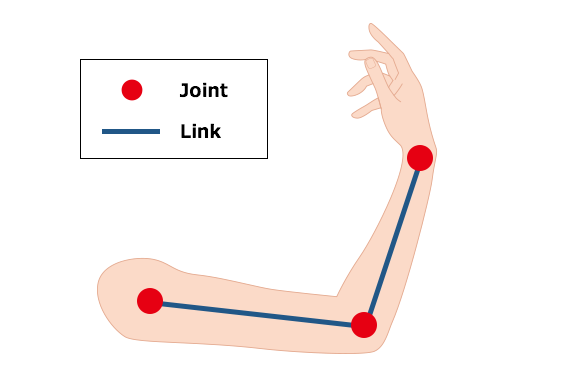
\includegraphics[width=\linewidth]{figures/arm.png}
	\caption{Single arm example}
	\label{fig:arm}
\end{figure}

Since robotics environments tend to be very complex especially in the real world and using actual hardware components, simulated engines had been selected to be programmed and simulate a robotic environment. This can then be transferred into real-world implementation with actual robotic arms and trained reinforcement learning agents. 

To understand the learning process in robotics environments, Inverse Kinematics (IK) need to be explained. The typical approach to learning to solve goals in robotics environments is using Inverse Kinematics which is defined as given a desired end-effector pose (position + orientation), find the values of the joint variables that will realize it. Meaning that given an end position for an effector, find the forces needed to be applied on joints to make the end effector reach it.

In robotic systems, the tasks are usually defined in coordinate space, whereas the control commands are defined in actuator space. In order to perform task-level robot learning, an appropriate transformation from coordinate space to actuator space is required. If the intrinsic coordinates of a manipulator are defined as a vector of joint angles \(\boldsymbol{\theta} \in \mathbf{R}^{\mathbf{n}}\), and the position and orientation vector of the end effector as a vector \(\mathbf{x} \in \mathbf{R}^{\mathrm{m}}\), then the forward kinematics function can be given by the following equation 
\begin{equation}
	        \mathbf{x}=f(\boldsymbol{\theta}).
\end{equation}

The inverse kinematics problem~\parencite{colome2011smooth, chua2013robust} is to find a mapping from the end-effector coordinates to actuator space which can be represented as
\begin{equation}
	        \boldsymbol{\theta}=f^{-1}(\mathbf{x}).
\end{equation}

Inverse kinematics for humanoid robots are important for many applications. Unlike closed-form analytical methods, the convergence time of numerical methods may vary and the results are not repeatable. On top of that, computing inverse kinematics under constraints of stability and self-collision avoidance cannot be done efficiently in real-time.

Using RL provide us many frameworks for not only learning the complex problem of IK but also to optimize the required criteria. Reinforcement Learning works on the experienced data and thus would avoid problems due to matrix inversions which may occur while solving general inverse kinematics. Therefore, learning would never demand impossible postures which occurs due to ill-conditioned matrix inversions. A general method to solve goal-oriented problems in robotics in a fairly general fashion. The desired goal \textit{(reward function)} for the robot need to be defined to solve the required task. In our environments, two reward functions are defined. One is used to make the finger of the robotic arm reach a certain sphere goal which is the target of the environment. The other one is modified in a way that keeps the target sphere move in the environment and the goal is to keep the arm following it as much as possible. 


\section{Software}
In this section, a description of the platforms used for the environment is provided along with specifying the APIs and the differences between the platforms and how they will be unified in our implementation. Then, we discuss the framework used for distribution and running reinforcement learning experiments. Stating the features provided by the framework and the modifications we have implemented to use it with our experiments. 

\subsection{Environment Platforms}

In the following, description of platforms used for the experiments is provided. The platforms interfaces are described, focusing on the advantages and differences between them and how to unify the platforms to run smoothly with the distributed framework to provide a stable baseline to compare between them.

\subsubsection{OpenAI Gym~\parencite{brockman2016openai}: } openai gym is a toolkit for developing and comparing reinforcement learning algorithms. It consists of a growing suite of environments (from simulated robots to Atari games), and a site for comparing and reproducing results. It supports teaching agents everything from walking to playing games like Pong or Pinball. The toolkit aims to accelerate reinforcement learning research. It has an open-source interface to reinforcement learning tasks which provides an easy-to-use suite of reinforcement learning tasks. The lack of standardization of environments used in publications and the need for better benchmarks were the main reasons the toolkit was developed to fix these problems.

The core gym interface~\ref{tab:gym_api} is \textbf{Env}, which is the unified environment interface. 
The following are the methods for the abstracted gym Env:

\begin{table}[!htb]
	\centering
	\begin{tabular}{|c|l|c|l|l|}
		\hline
		\multicolumn{5}{|c|}{\textbf{OpenAI Gym API Interface}}                                                                                                                                                                                      \\ \hline
		\multicolumn{2}{|c|}{\textit{\textbf{Function}}}                                  & \multicolumn{3}{c|}{\textit{\textbf{Description}}}                                            \\ \hline
		\multicolumn{2}{|c|}{\cellcolor[HTML]{E6E6E6}\textbf{reset(self)}}                & \multicolumn{3}{c|}{\textit{\begin{tabular}[c]{@{}c@{}}Reset the environment's state.         \\ Returns observation.\end{tabular}}}                             \\ \hline
		\multicolumn{2}{|c|}{\cellcolor[HTML]{E6E6E6}\textbf{step(self, action)}}         & \multicolumn{3}{c|}{\textit{\begin{tabular}[c]{@{}c@{}}Step the environment by one time-step. \\ Returns observation, reward, done, info.\end{tabular}}} \\ \hline
		\multicolumn{2}{|c|}{\cellcolor[HTML]{E6E6E6}\textbf{render(self, mode='human')}} & \multicolumn{3}{c|}{\textit{Render one frame of the environment.}}                            \\ \hline
	\end{tabular}
	\caption{OpenAI Gym API Interface}
	\label{tab:gym_api}
\end{table}

\subsubsection{Unity MLAgents~\parencite{juliani2018unity}: }\label{unity_mlagents} Unity mlagents toolkit is an open-source Unity plugin that enables games and simulations to serve as environments for training intelligent agents. It has a more realistic and complex simulation environment. It provides the ability to flexibly configure
the simulation. By taking advantage of Unity as a simulation platform, the toolkit enables the development of learning environments which are rich in sensory and physical complexity, provide compelling cognitive challenges, and support dynamic multi-agent interaction. Agents can be trained using reinforcement learning, imitation learning, neuroevolution, or other machine learning methods through a simple to use Python API. They provide implementations of state-of-the-art algorithms to enable game developers and hobbyists to easily train intelligent agents for 2D, 3D, and VR/AR games. We are using this to test running multiple agents in the same environment and compare the effect with one agent only. Also, to experiment with the transferability between different physics simulators.

The learning environment is quite different from openai gym as it consists of three main components described below:

\begin{itemize}
	\item \textbf{Agent:} Each Agent can have a unique set of states and observations, take unique actions within the environment, and receive unique rewards for events within the environment. An agent’s actions are decided by the brain it is linked to.
	\item \textbf{Brain:} Each Brain defines a specific state and action space and is responsible for deciding which actions each of its linked agents will take. The supported brains mode are External, Internal, Player, Heuristic. \textit{\textbf{In our experiments, External mode is used as the action decisions are made using ML library through communication over an open socket with Python API.}}
	\item \textbf{Academy:} The Academy object within a scene also contains as children all Brains within the environment. Each environment contains a single Academy which defines the scope of the environment, in terms of: Engine Configuration, Frame-skip \& Global episode length
\end{itemize}

\begin{figure}[!htb]
	\centering
	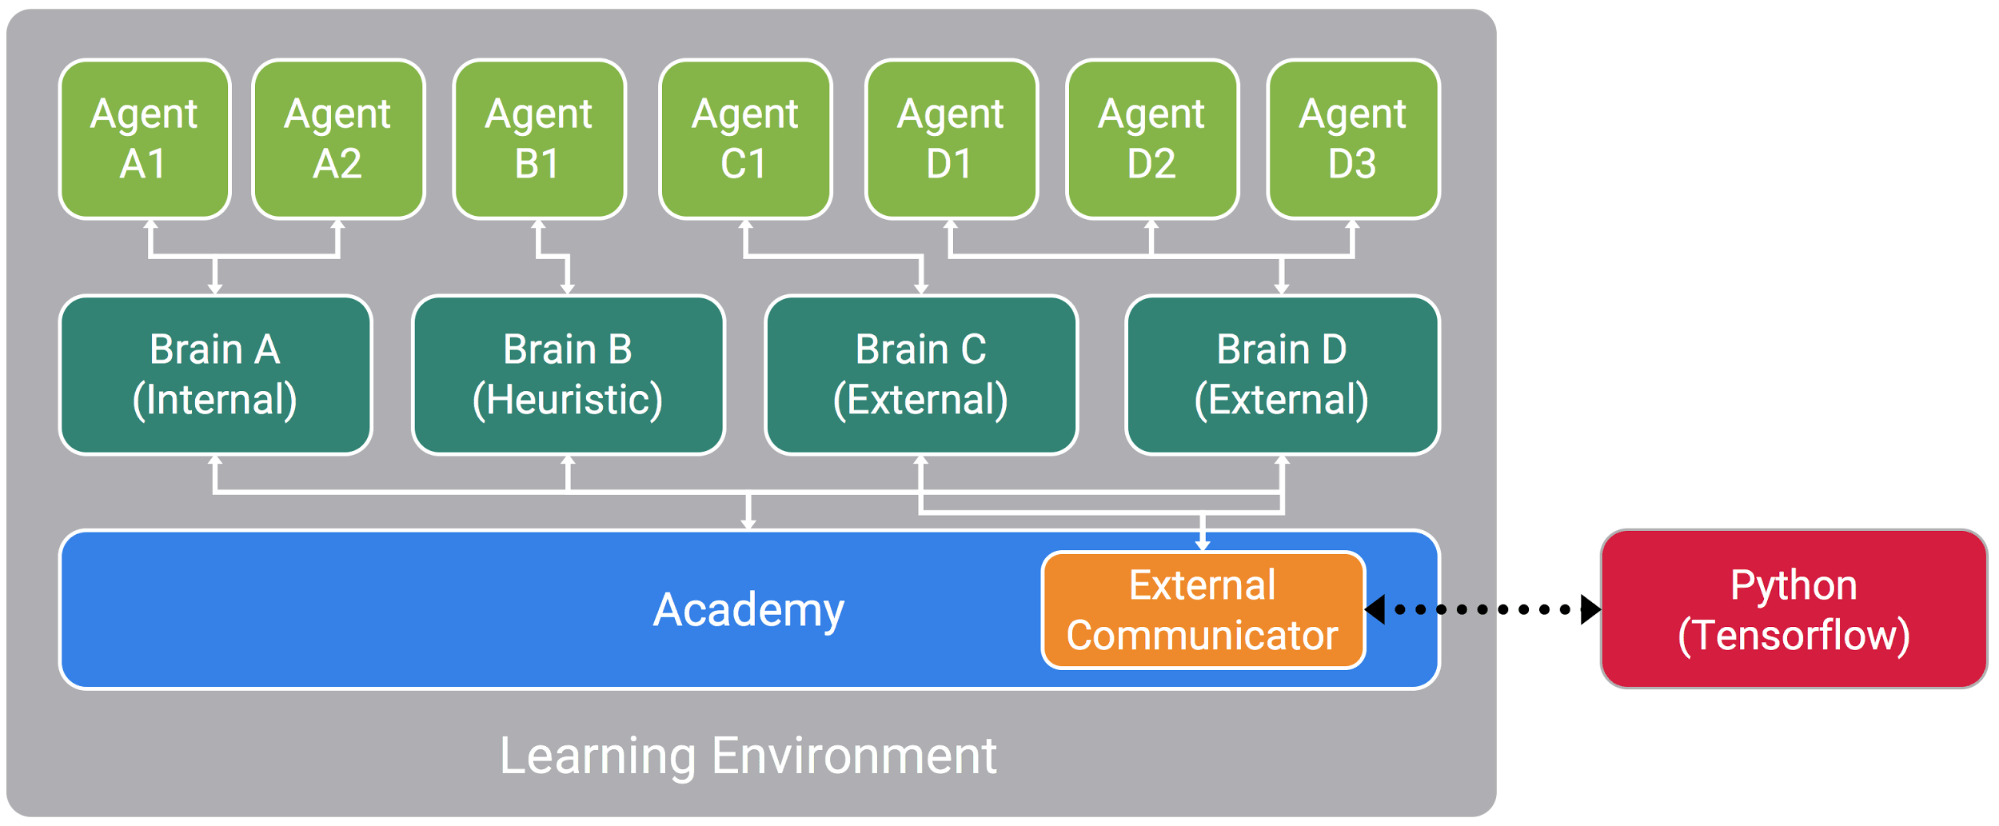
\includegraphics[width=\linewidth]{figures/unity_api.png}
	\caption{Unity Learning Environment Architecture}
	\label{fig:unity_api}
\end{figure}

The states and observations of all agents with brains set to External are collected by the External Communicator and communicated to our Python API for processing using your ML library of choice. By setting multiple agents to a single brain, actions can be decided in a batch fashion, opening the possibility of getting the advantages of parallel computation, when supported.

Unity ML-Agents toolkit provides a variety of training scenarios are possible, depending on how agents, brains, and rewards are connected. Scenarios include Single-Agent (A single agent linked to a single brain), Simultaneous Single-Agent (Multiple independent agents with independent reward functions linked to a single brain, providing a parallelized version of the traditional training scenario, which can speed-up and stabilize the training process), Adversarial Self-Play (Two interacting agents with inverse reward functions linked to a single brain), Cooperative Multi-Agent (Multiple interacting agents with a shared reward function linked to either a single or multiple different brains) and Ecosystem (Multiple interacting agents with independent reward function linked to either a single or multiple different brains).

\subsection{Distributed Ray Framework}

\textbf{Ray~\parencite{moritz2018ray}} is a fast and simple framework for building and running distributed applications. The same code can be run on a single machine to achieve efficient multiprocessing, and it can be used on a cluster for large computations. Ray provide high scalability and a unified API for a variety of applications which is very useful for our experiments. Ray executes tasks asynchronously to achieve parallelism enabling us to run multiple environments in the same experiment to benefit from collection more experiences and trajectories for the agent.

As a distributed computing system, Ray still follows the typical Master-Slave design appeared in Figure~\ref{fig:ray_arch} below: Master is responsible for global coordination and state maintenance, and Slave performs distributed computing tasks. However, unlike traditional distributed computing systems, Ray uses the idea of \textbf{hybrid task scheduling}. In cluster deployment mode, Ray starts the following key components:

\begin{itemize}
	\item \textbf{Global Scheduler:} A global scheduler is started on the Master to receive the tasks submitted by the local scheduler and distribute the tasks to the appropriate local task scheduler for execution.
	\item \textbf{Redis Server:} One or more redis servers are started on the Master to save the state information (ControlState) of distributed tasks, including object machine mapping, task description, task debug information, and so on.
	\item \textbf{Local Scheduler:} A local scheduler is started on each slave to submit tasks to the global scheduler and assign tasks to the current machine's Worker process.
	\item \textbf{Worker:} Multiple worker processes can be started on each slave to perform distributed tasks, and the calculation results are stored in the ObjectStore.
	\item \textbf{Object Store:} An object store storage read-only data object is started on each Slave. Workers can access these object data through shared memory, which can effectively reduce the cost of memory copy and object serialization. The underlying ObjectStore is implemented by Apache Arrow.
	\item \textbf{Plasma:} The object store on each slave is managed by an object manager called Plasma. It can actively pull object data from other slaves to the current machine when the worker accesses remote data objects that do not exist on the local ObjectStore.
\end{itemize}

\begin{figure}[!htb]
	\centering
	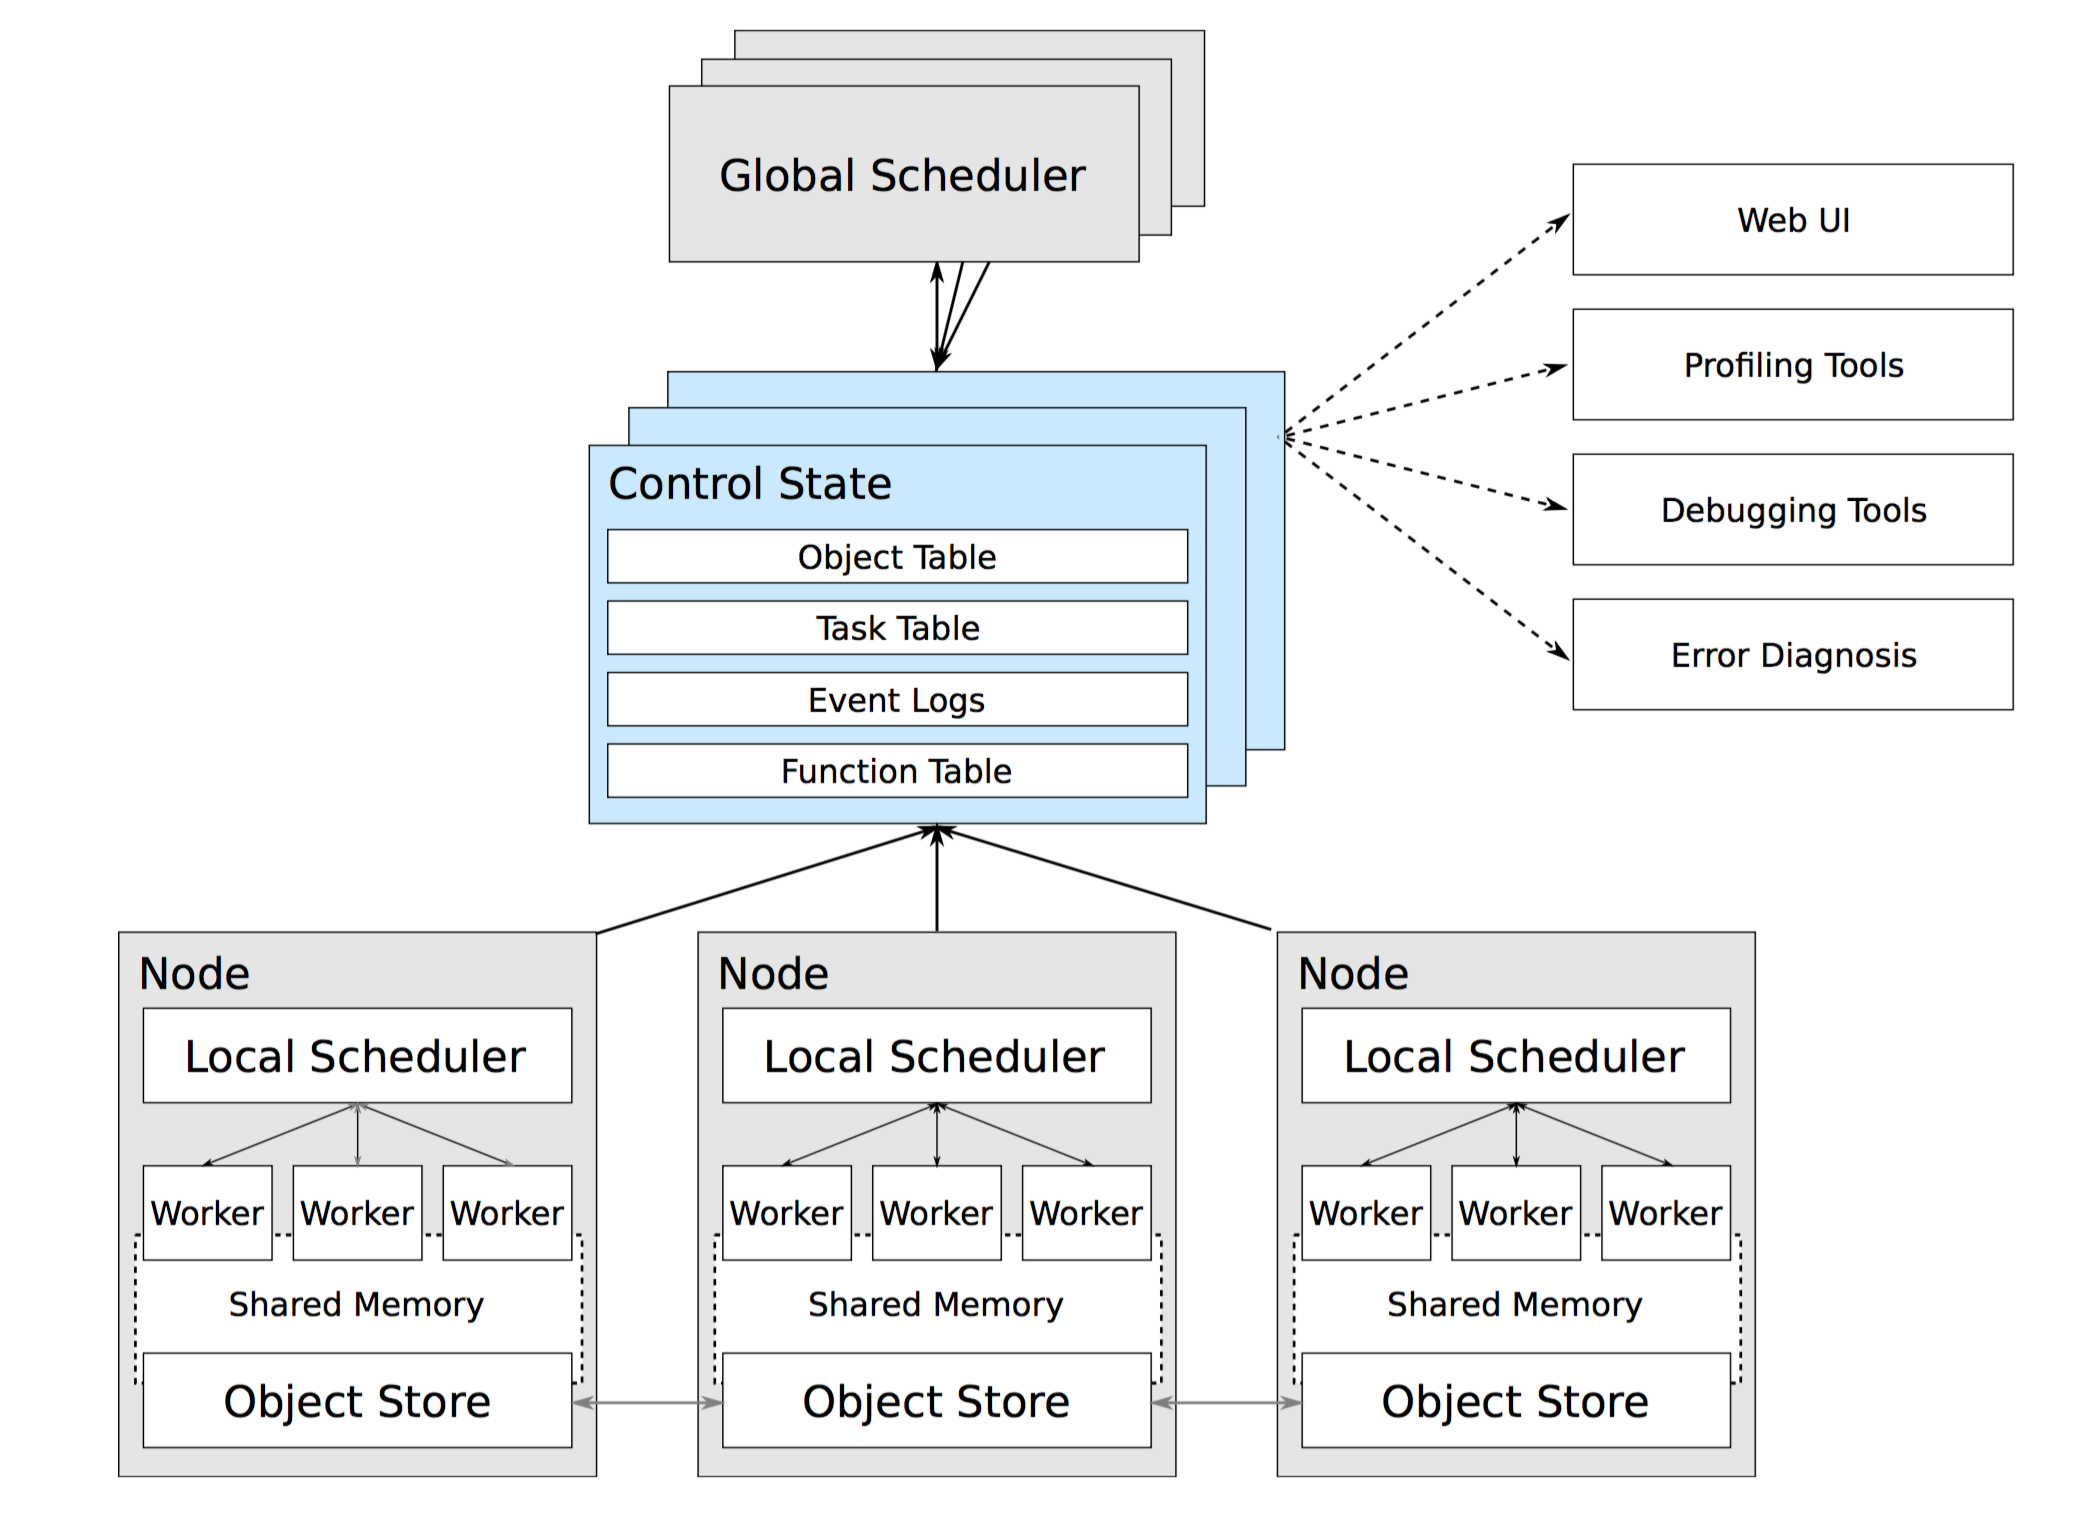
\includegraphics[width=\linewidth]{figures/ray_arch.png}
	\caption{Ray's system architecture}
	\label{fig:ray_arch}
\end{figure}



\section{Architecture}

The structure of reinforcement learning computations as shown in the figure~\ref{fig:rl_computation} below, follows a simple abstract approach where the environment send states (observations) to the agent and the agent transform the states to proper actions. The focus here in the Agent computation, how to speed up this process, from storing the trajectories (experiences) from the environment to computing the stochastic gradient descent and improving the policy till policy evaluation and converting the states to actions. Since most reinforcement learning algorithms share common components like (the Policy \(\pi_{\theta}\left(S_{t}\right)\), Preprocessing Trajectory \(\rho_{\theta}(X)\), and Loss functions \(L(\theta, X)\)), there is a need to unify these component among different algorithms to have a system that effectively meet all the varied demands of RL workloads.
\begin{figure}[!htb]
	\centering
	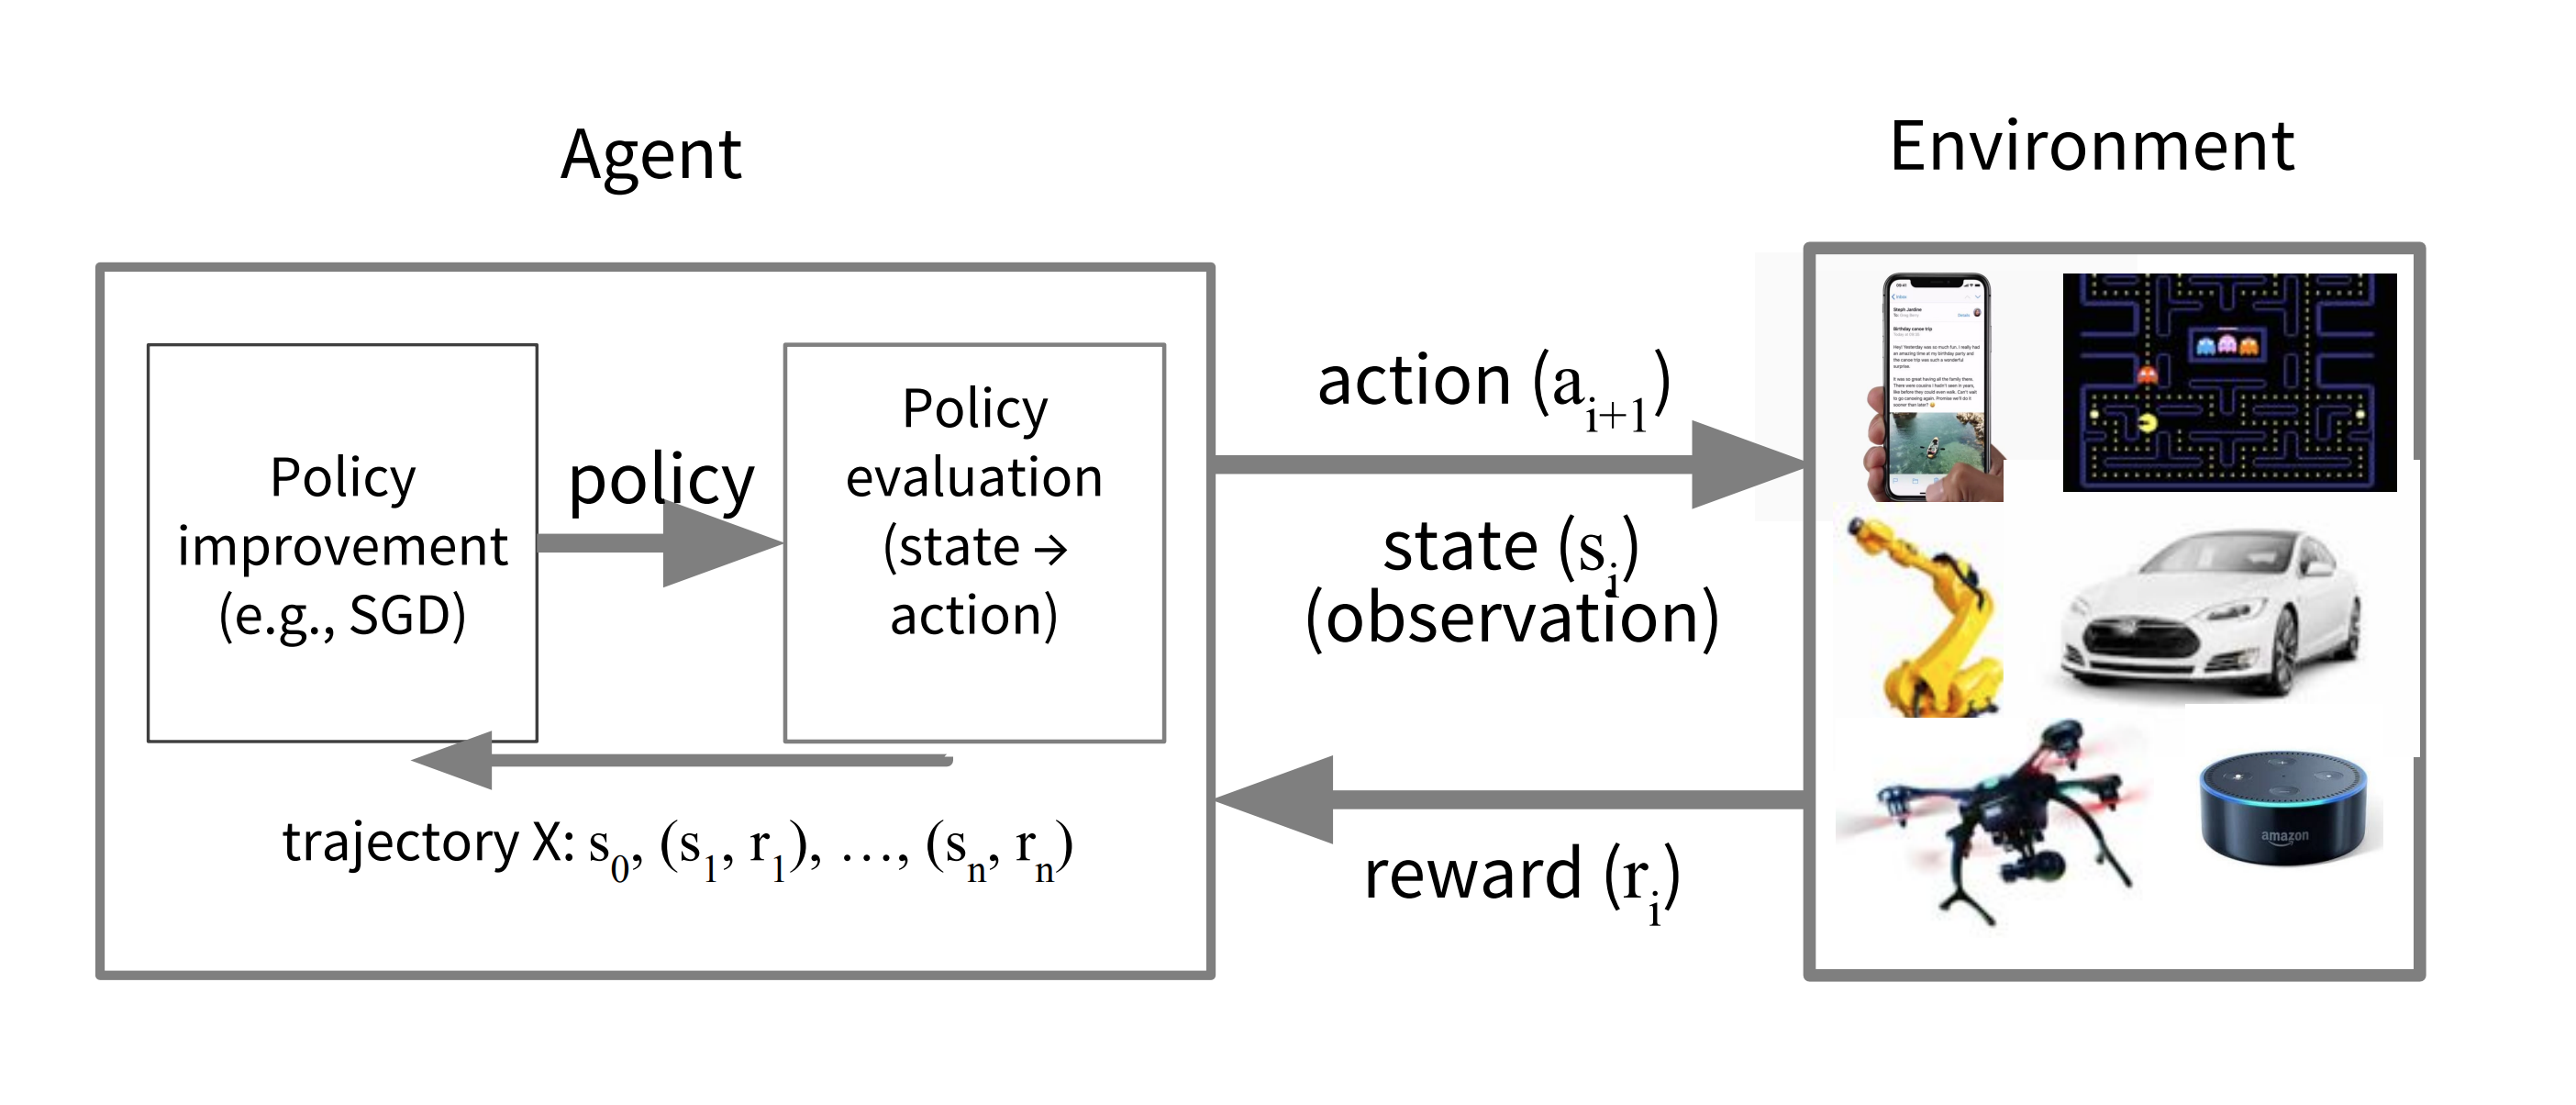
\includegraphics[width=\linewidth]{figures/architecture/rl_computation.png}
	\caption{Structure of RL computations}
	\label{fig:rl_computation}
\end{figure}

In order to meet the requirements and provide enhanced learning scenario, there is a needs to support stateful computations (for environment simulators, neural networks, replay buffers), support heterogeneous computing tasks, dynamically compute links, millisecond-level latency, allow easy composition of (distributed) components, and the ability to schedule millions of tasks per second. This is provided by a higher-level RL abstractions which enable hierarchical parallel task model, as shown in the figure~\ref{fig:rl_htm}, with stateful workers that is flexible enough to capture a broad range of RL workloads 
\begin{figure}[!htb]
	\centering
	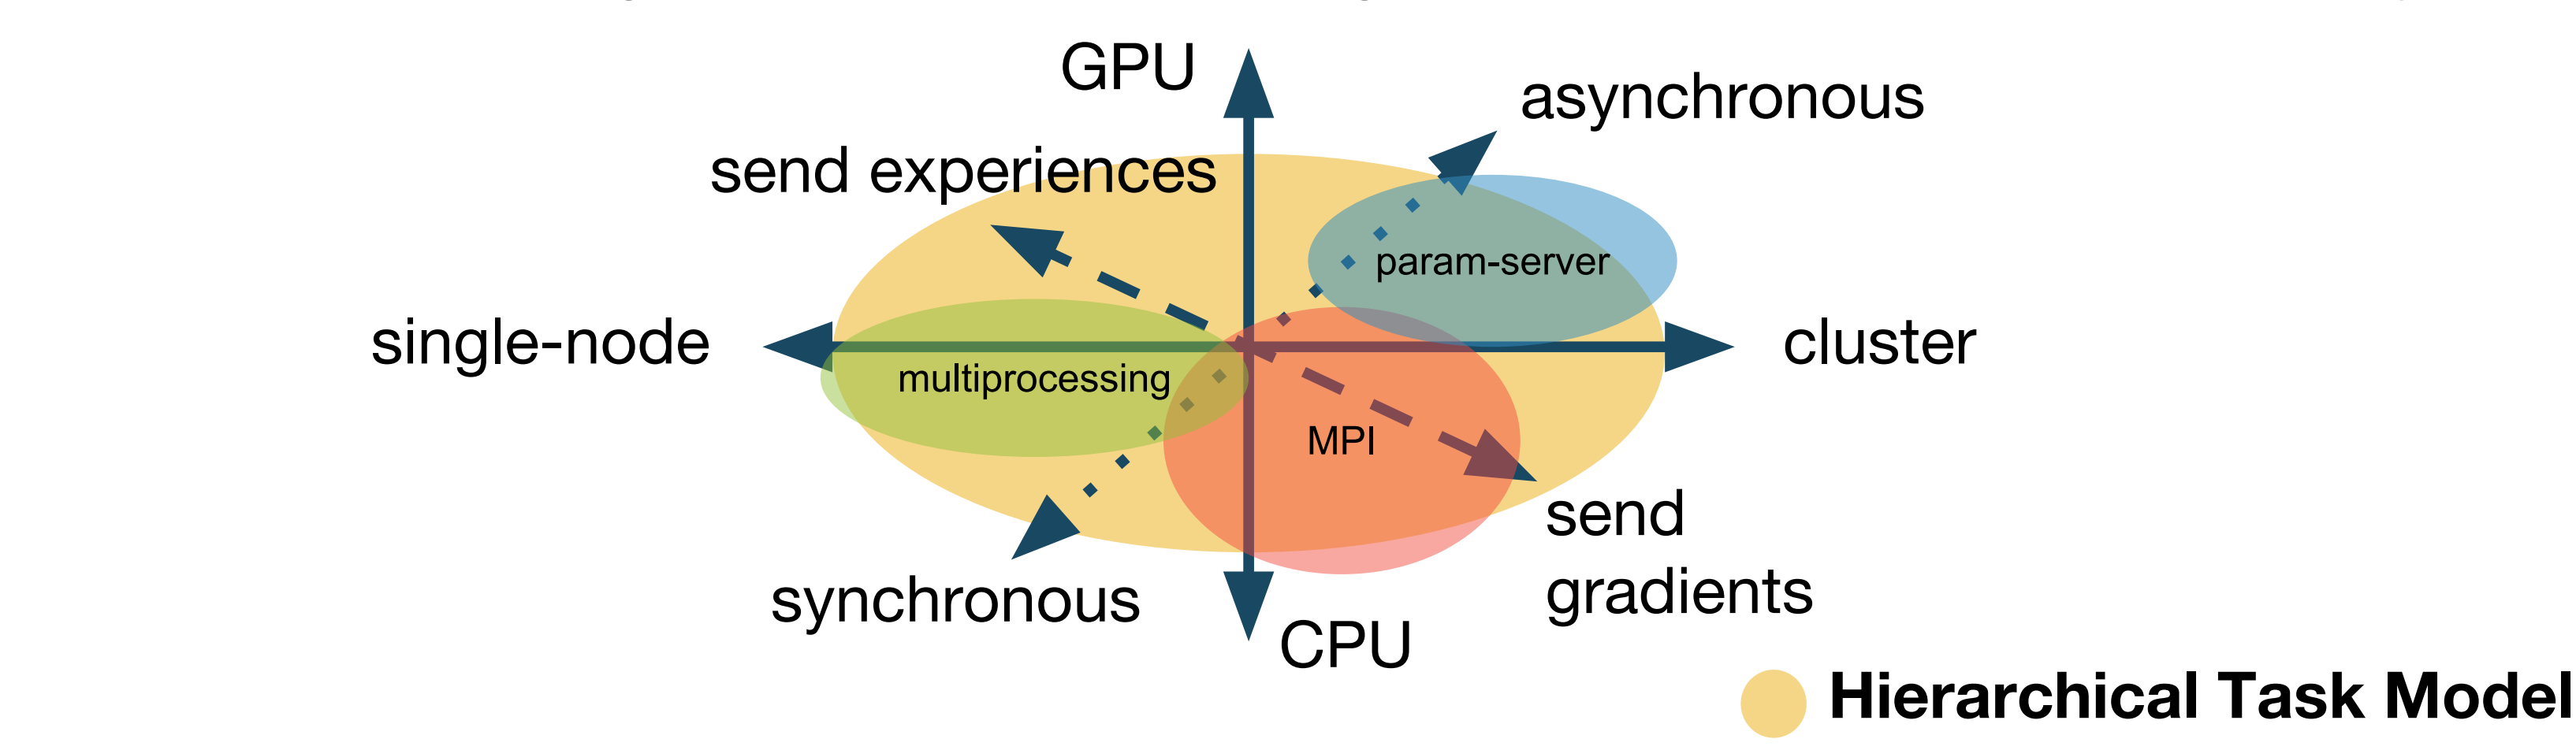
\includegraphics[width=\linewidth]{figures/architecture/htm.png}
	\caption{Hierarchical Task Model}
	\label{fig:rl_htm}
\end{figure}

Using the \textbf{Hierarchical Parallel Task Model}, it is easy to create python class instances in the ray cluster (representing the stateful workers), enabling running multiple training steps, collecting experiences from the environment, using all-reduce for the gradient optimization and exchange weight shards through Ray object store. The following Figure~\ref{fig:ray_cluster} an illustration for the ray cluster components.
\begin{figure}[!htb]
	\centering
	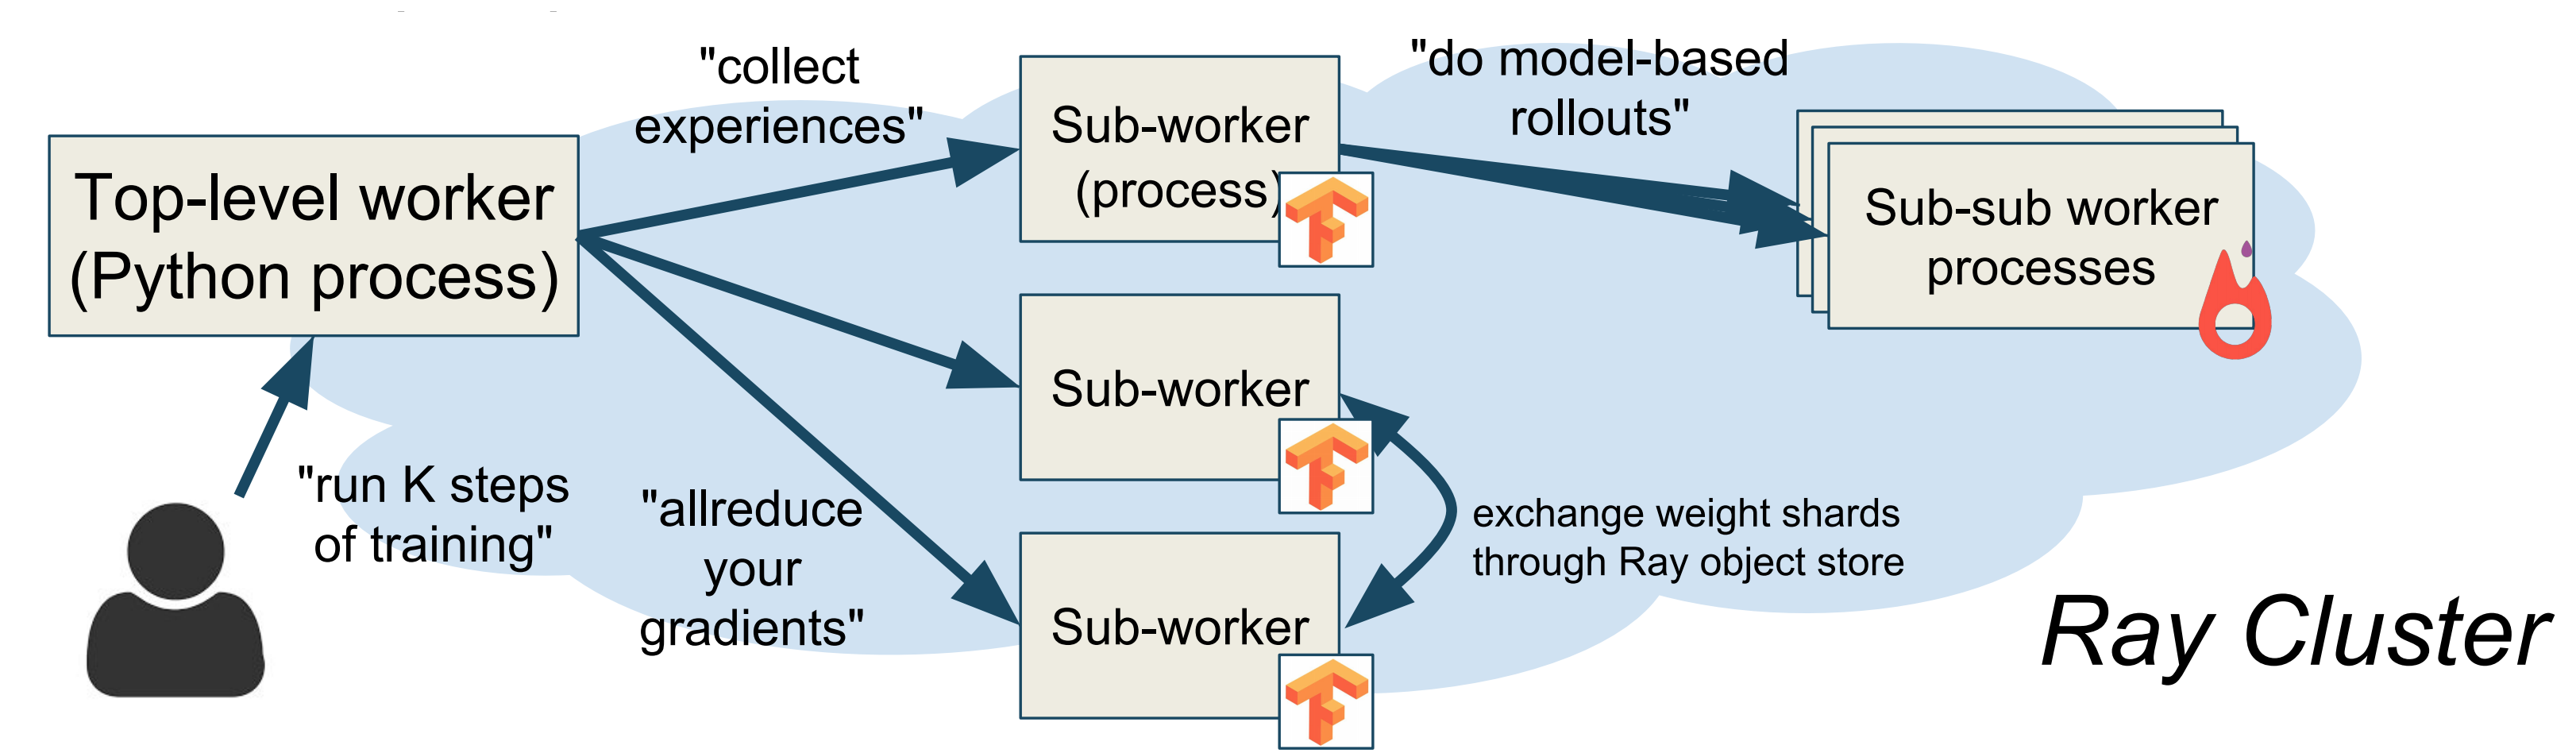
\includegraphics[width=\linewidth]{figures/architecture/ray_cluster.png}
	\caption{Ray Cluster}
	\label{fig:ray_cluster}
\end{figure}

Ray distributed execution engine shown in Figure~\ref{fig:ray_engine}, provides \textbf{Task parallel} and \textbf{Actor APIs} built on \textbf{dynamic task graphs}. These APIs are used to build distributed applications, libraries and systems providing faster execution than python multiprocessing on a single node and competitive performance with MPI in many workloads.
\begin{figure}[!htb]
	\centering
	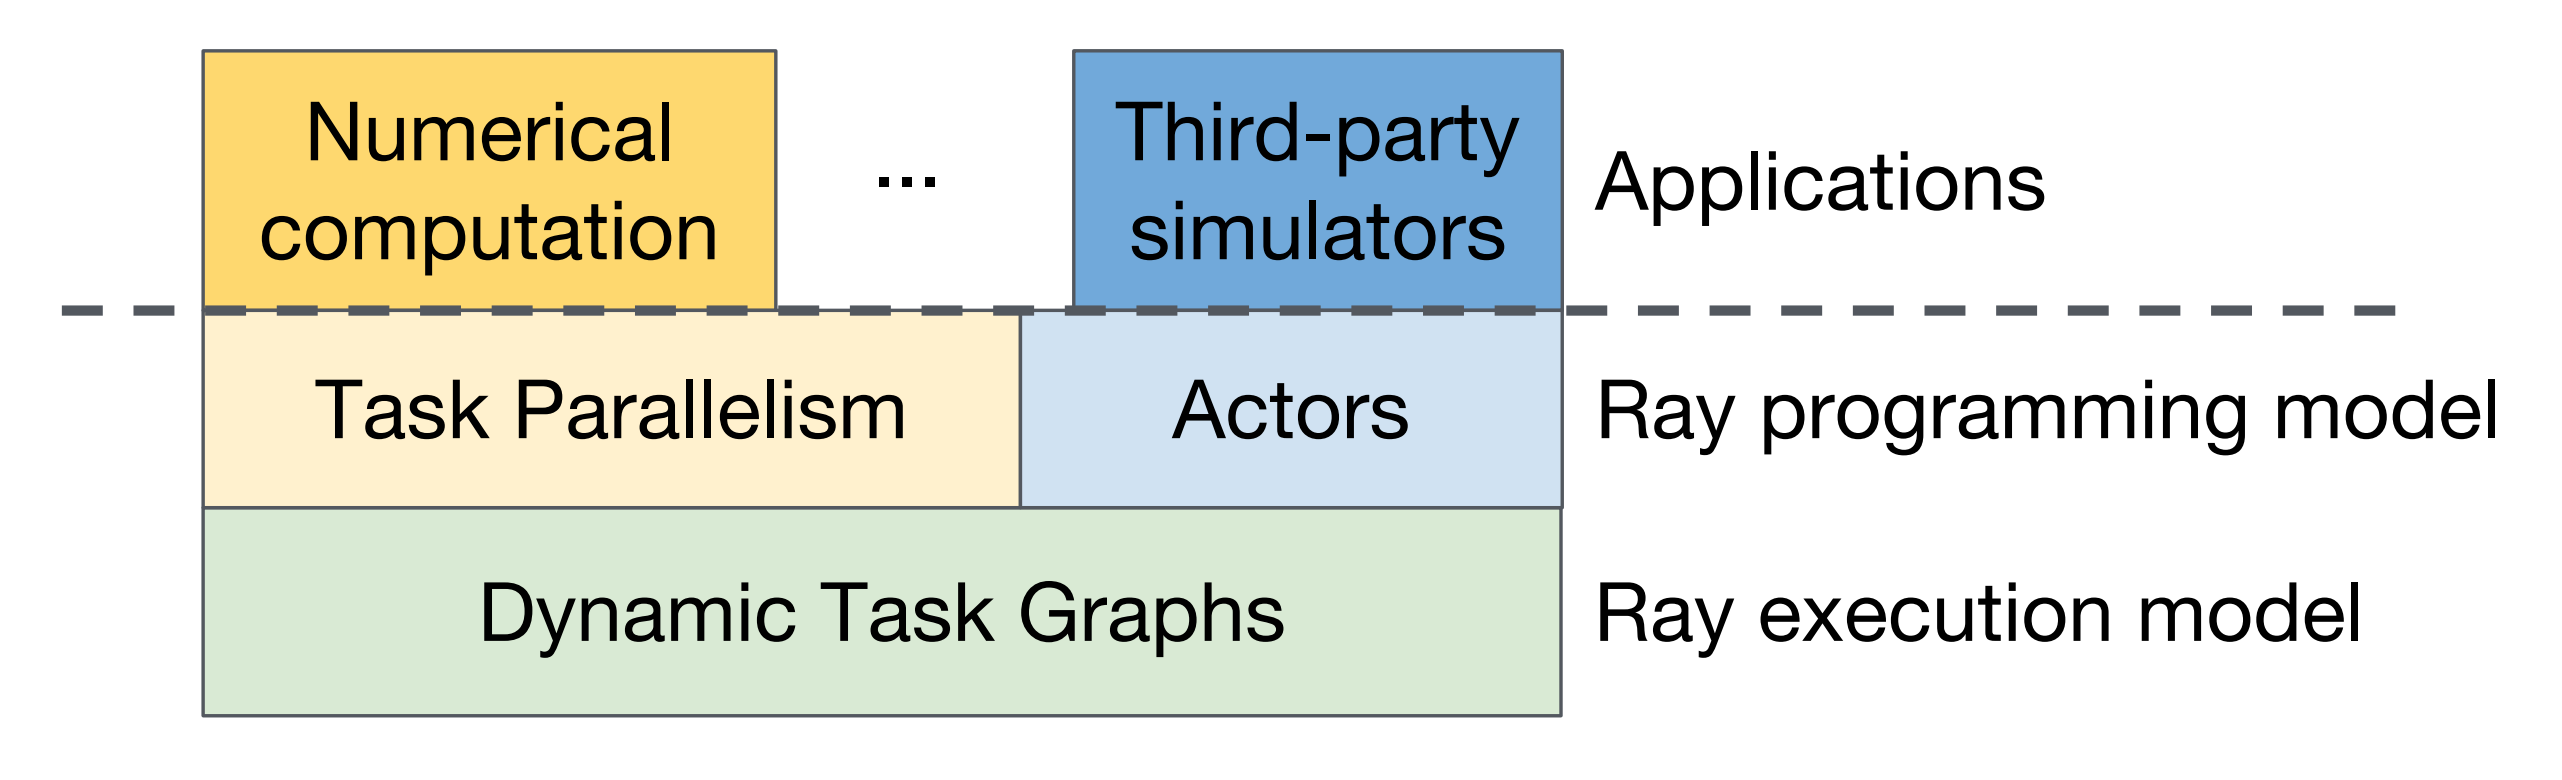
\includegraphics[width=\linewidth]{figures/architecture/ray_engine.png}
	\caption{Ray Distributed Execution Engine}
	\label{fig:ray_engine}
\end{figure}


At a high level, ray provides an \textbf{\colorbox{gray!20}{Trainer}} class which holds a policy for environment interaction. Through the trainer interface shown in Figure~\ref{fig:ray_trainer}, the policy can be trained, check-pointed, or an action computed. In multi-agent training, the trainer manages the querying and optimization of multiple policies at once. 
\begin{figure}[!htb]
	\centering
	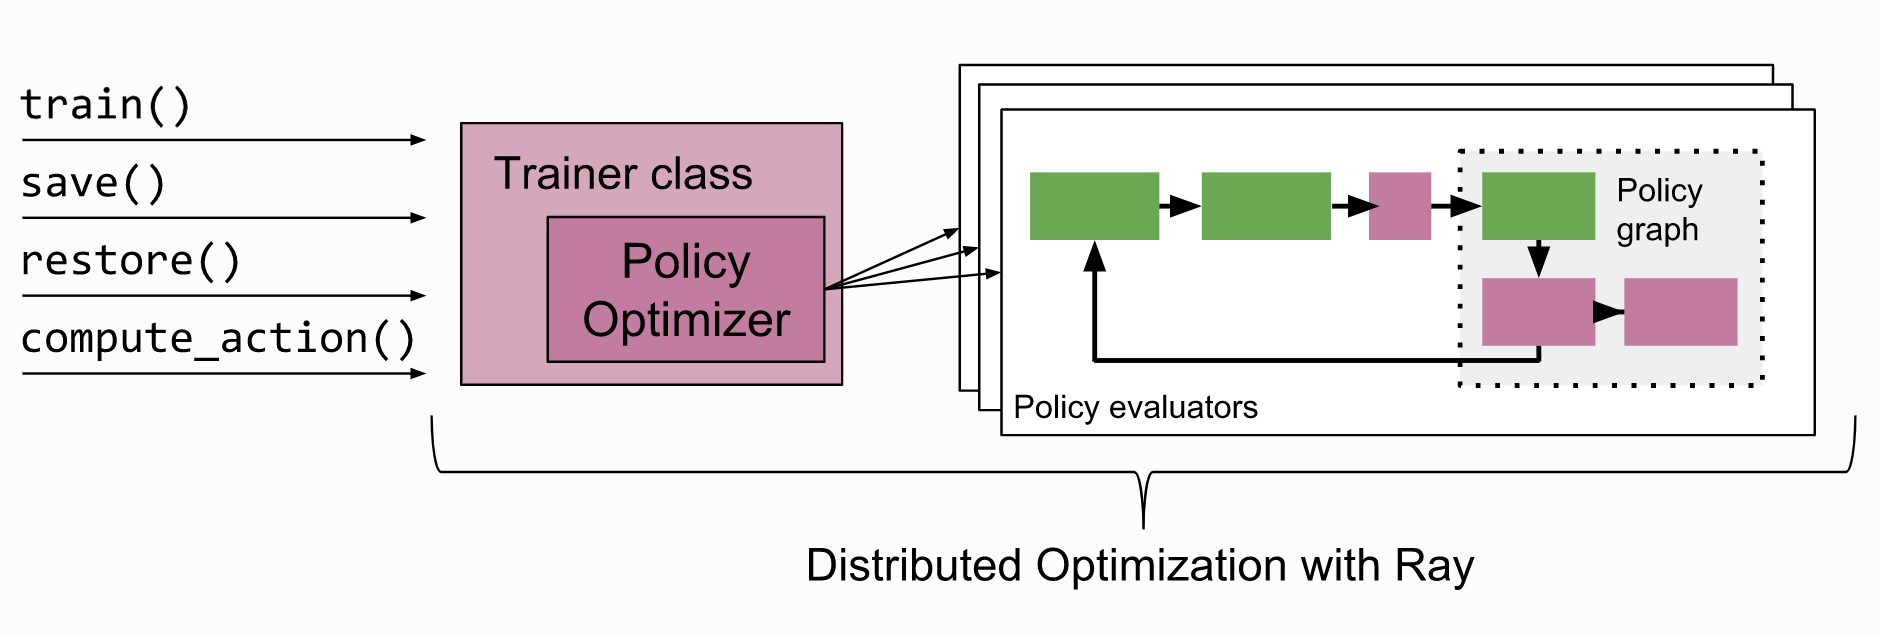
\includegraphics[width=\textwidth]{figures/architecture/ray_trainer.png}
	\caption{Ray Training Process}
	\label{fig:ray_trainer}
\end{figure}

It provides custom resources configurations~\ref{fig:ray_config}, which can control the degree of parallelism used by setting the \colorbox{gray!20}{\texttt{num\_workers}} hyper-parameter for most algorithms. The number of GPUs the driver should use can be set via the \colorbox{gray!20}{\texttt{num\_gpus}} option. Similarly, the resource allocation to workers can be controlled via \colorbox{gray!20}{\texttt{num\_cpus\_per\_worker}}, \colorbox{gray!20}{\texttt{num\_gpus\_per\_worker}}, and \colorbox{gray!20}{\texttt{custom\_resources\_per\_worker}}. The number of GPUs can be a fractional quantity to allocate only a fraction of a GPU. For example, with DQN you can pack five trainers onto one GPU by setting \colorbox{gray!20}{\texttt{num\_gpus}: 0.2}.
\begin{figure}[!htb]
	\centering
	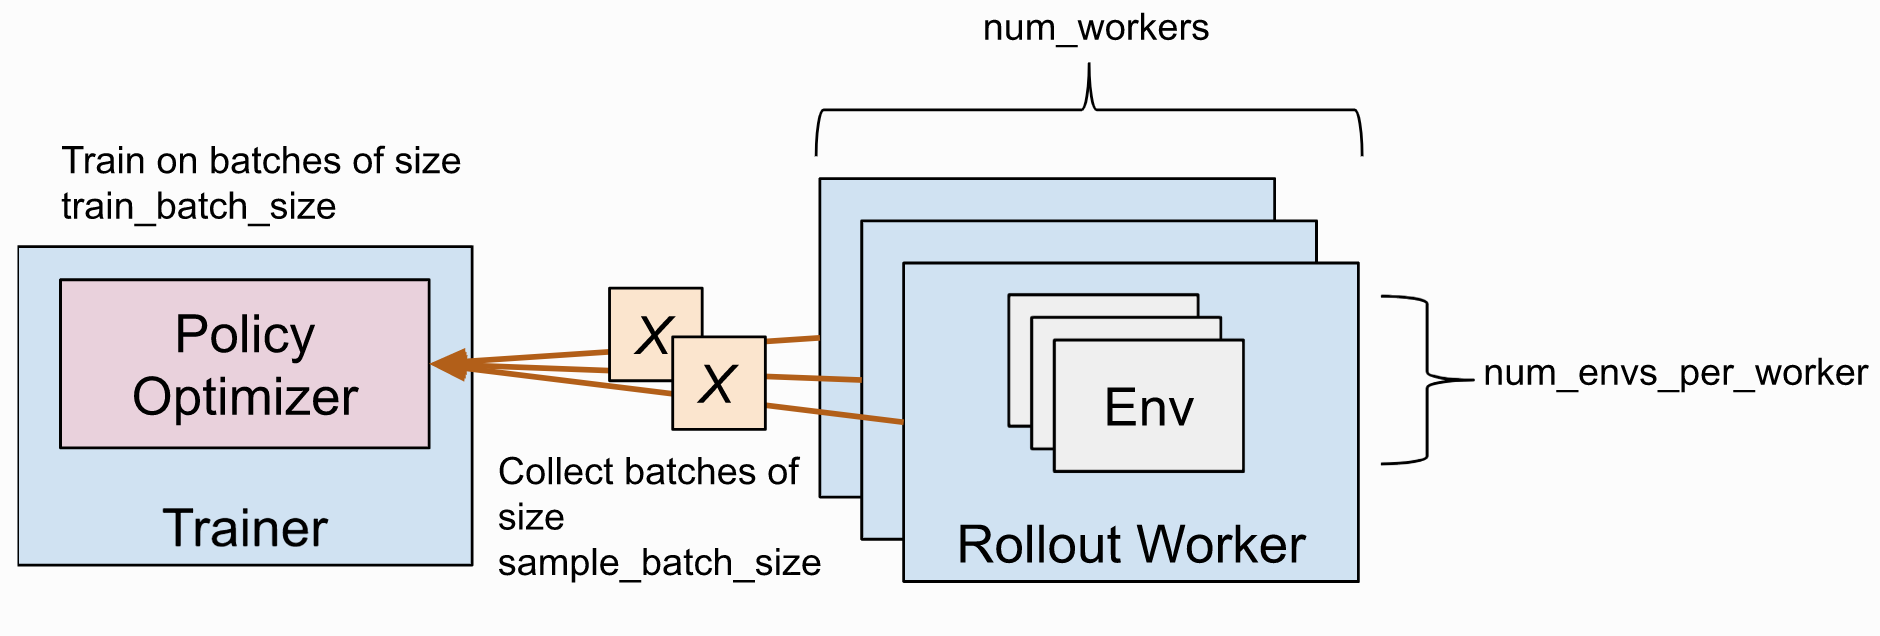
\includegraphics[width=\textwidth]{figures/architecture/ray_config.png}
	\caption{Ray Configurable resources}
	\label{fig:ray_config}
\end{figure}

The following diagram provides a conceptual overview of data flow between different components. It starts with an \colorbox{gray!20}{\texttt{Environment}}, which given an action produces an observation. The observation is preprocessed by a \colorbox{gray!20}{\texttt{Preprocessor}} and \colorbox{gray!20}{\texttt{Filter}} (for running mean normalization) before being sent to a neural network \colorbox{gray!20}{\texttt{Model}}. The model output is in turn interpreted by an \colorbox{gray!20}{\texttt{ActionDistribution}} to determine the next action.
\begin{figure}[!htb]
	\centering
	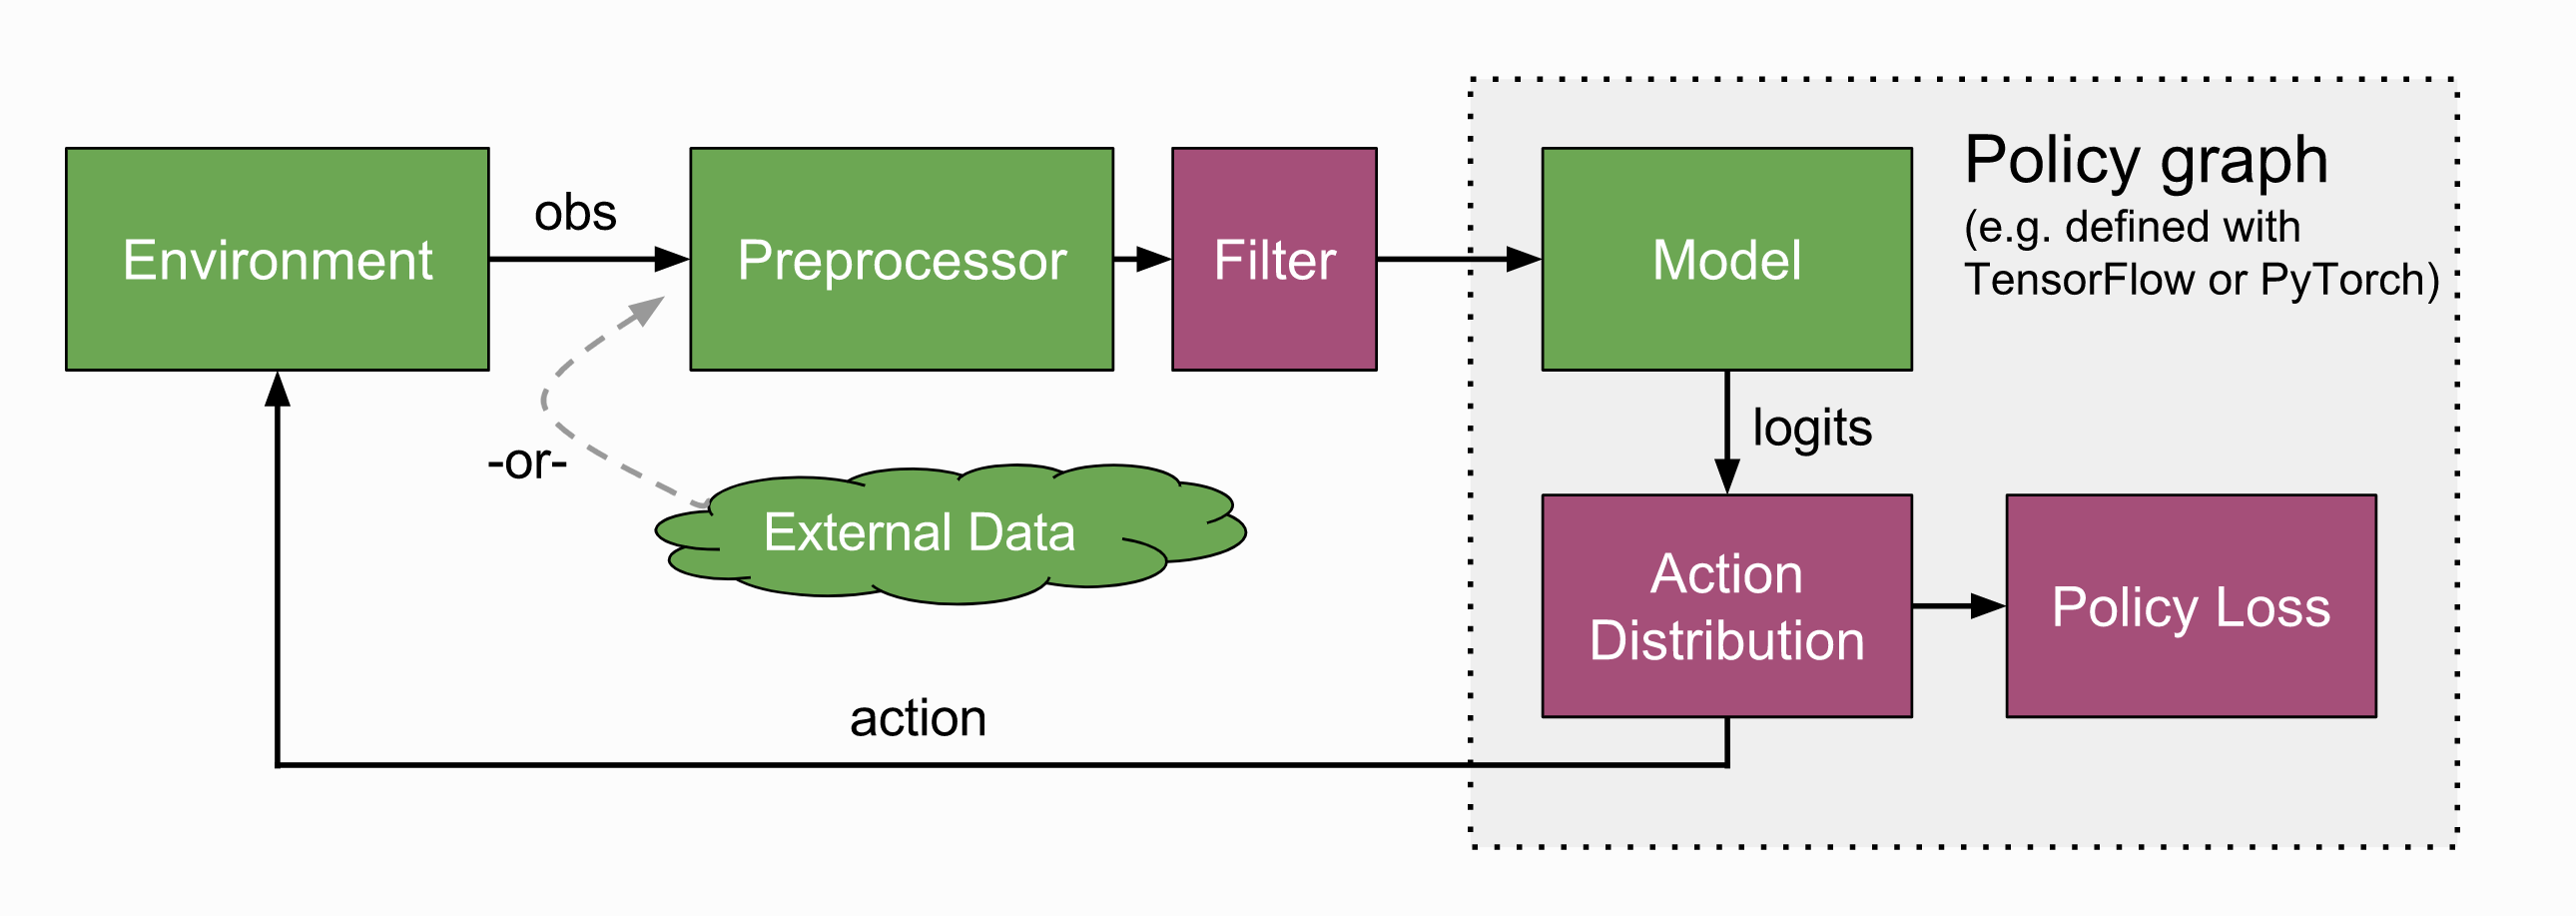
\includegraphics[width=\textwidth]{figures/architecture/ray_loop.png}
	\caption{Ray Conceptual Overview of Data Flow, Models, \& Preprocessors}
	\label{fig:ray_loop}
\end{figure}

To speed up rollouts for policy gradients, ray use simulators on CPUs, policies on GPUs. This enables parallel rollouts on CPU and improve policy evaluation on GPU which enable reaching speedup of \textbf{4.1x} for \textbf{fine grained rollouts} as shown in the following figure~\ref{fig:ray_speedup}.
\begin{figure}[!htb]
	\centering
	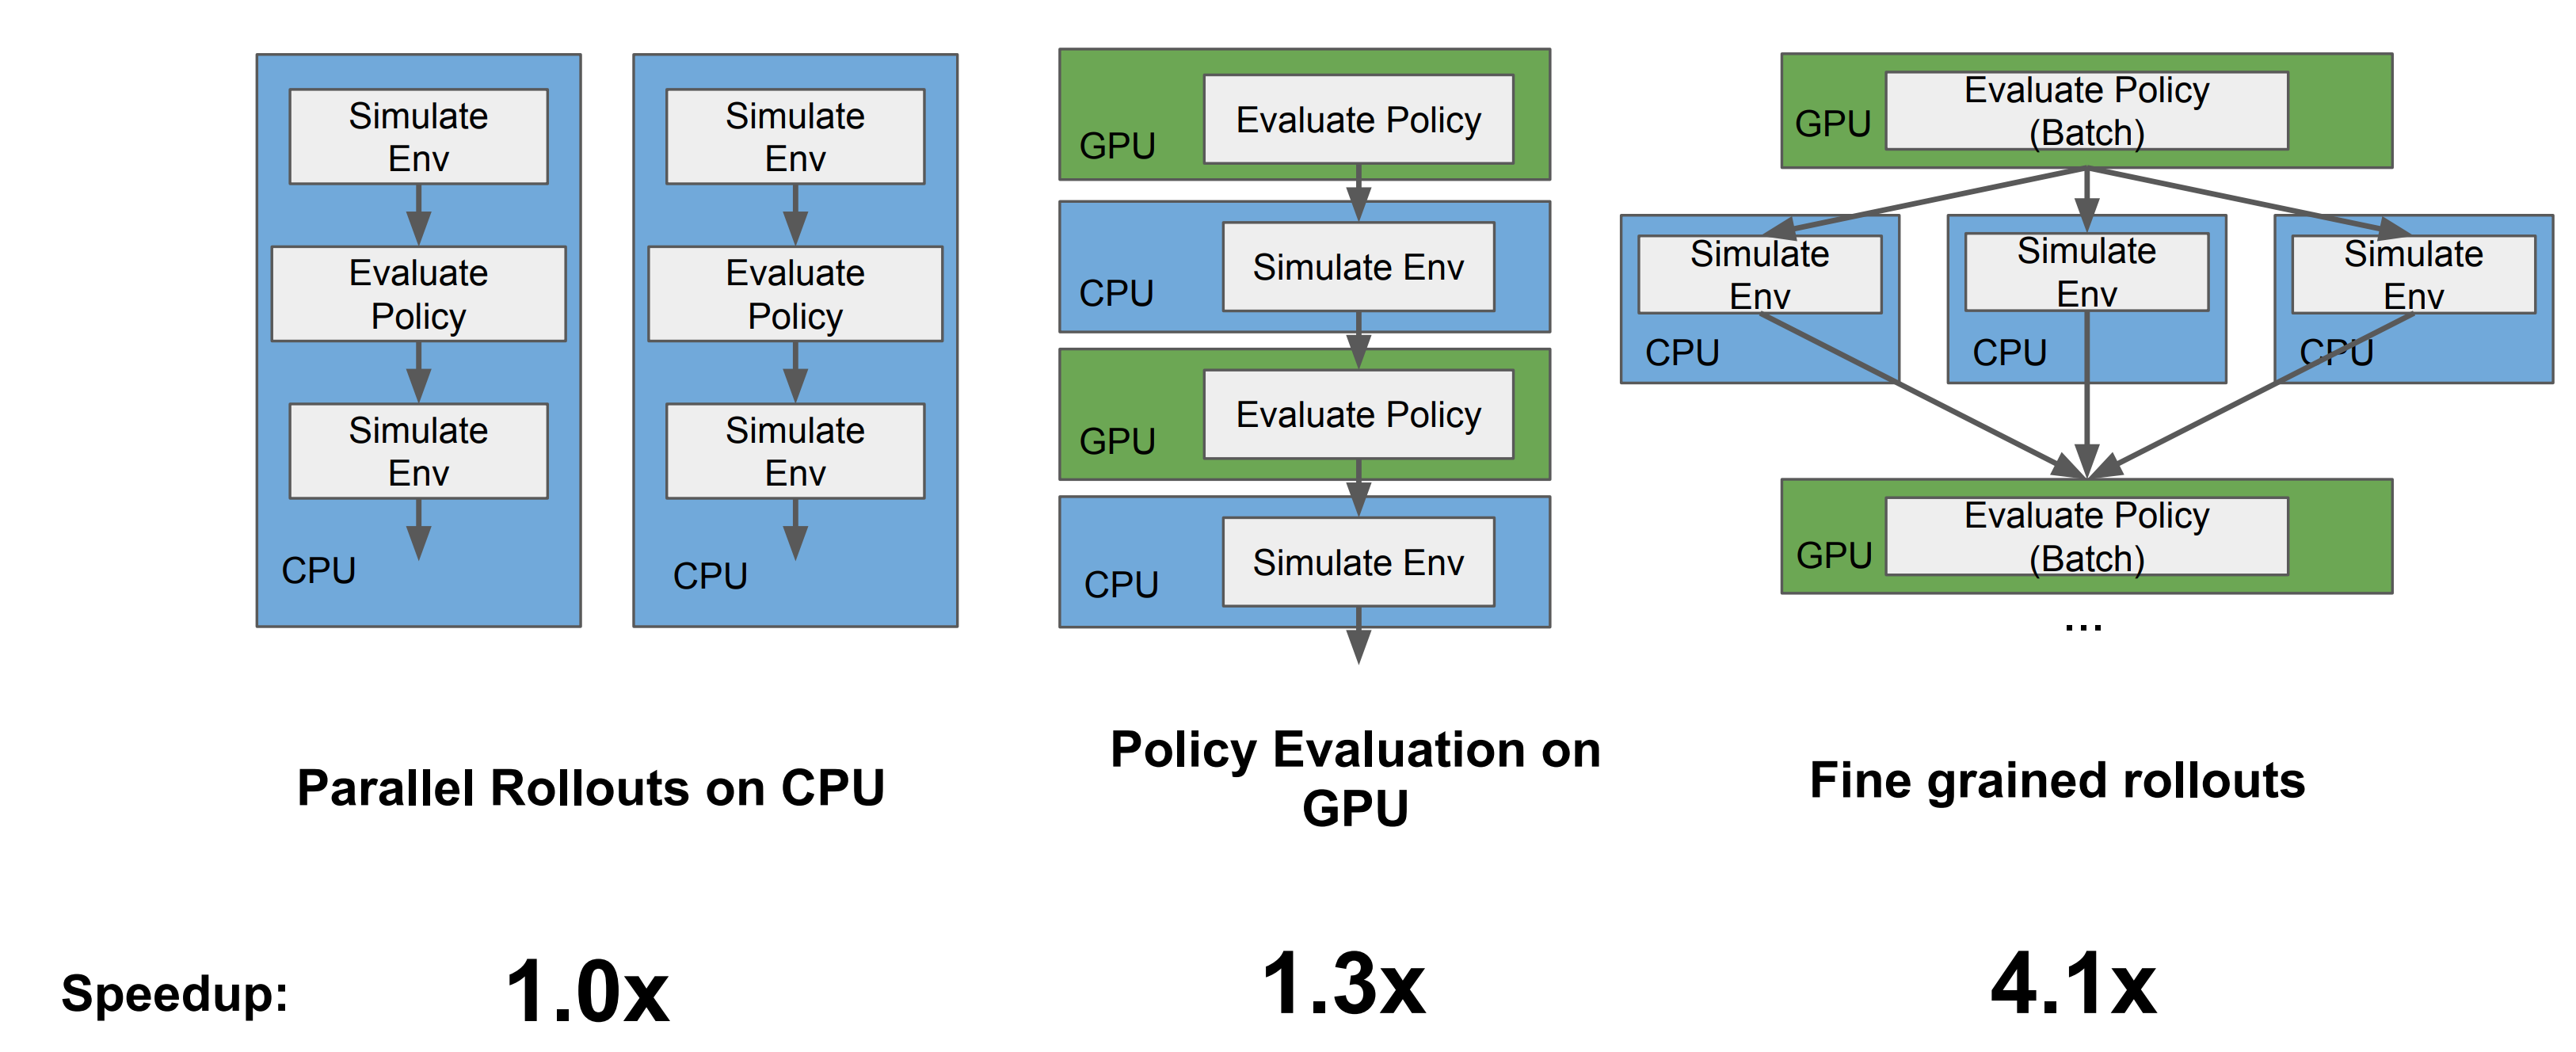
\includegraphics[width=\textwidth]{figures/architecture/ray_speedup.png}
	\caption{Speeding up rollouts for policy gradients}
	\label{fig:ray_speedup}
\end{figure}


Since ray support only OpenAI Gym environments along with their provided multi-agent and also batched environments, we had to implement our custom environment to unify between unity mlagents and openai gym environments. Also, we implemented our custom Multi-Agent environments for both used environments as shown in the following figure~\ref{fig:ray_envs}.

\begin{figure}[!htb]
	\centering
	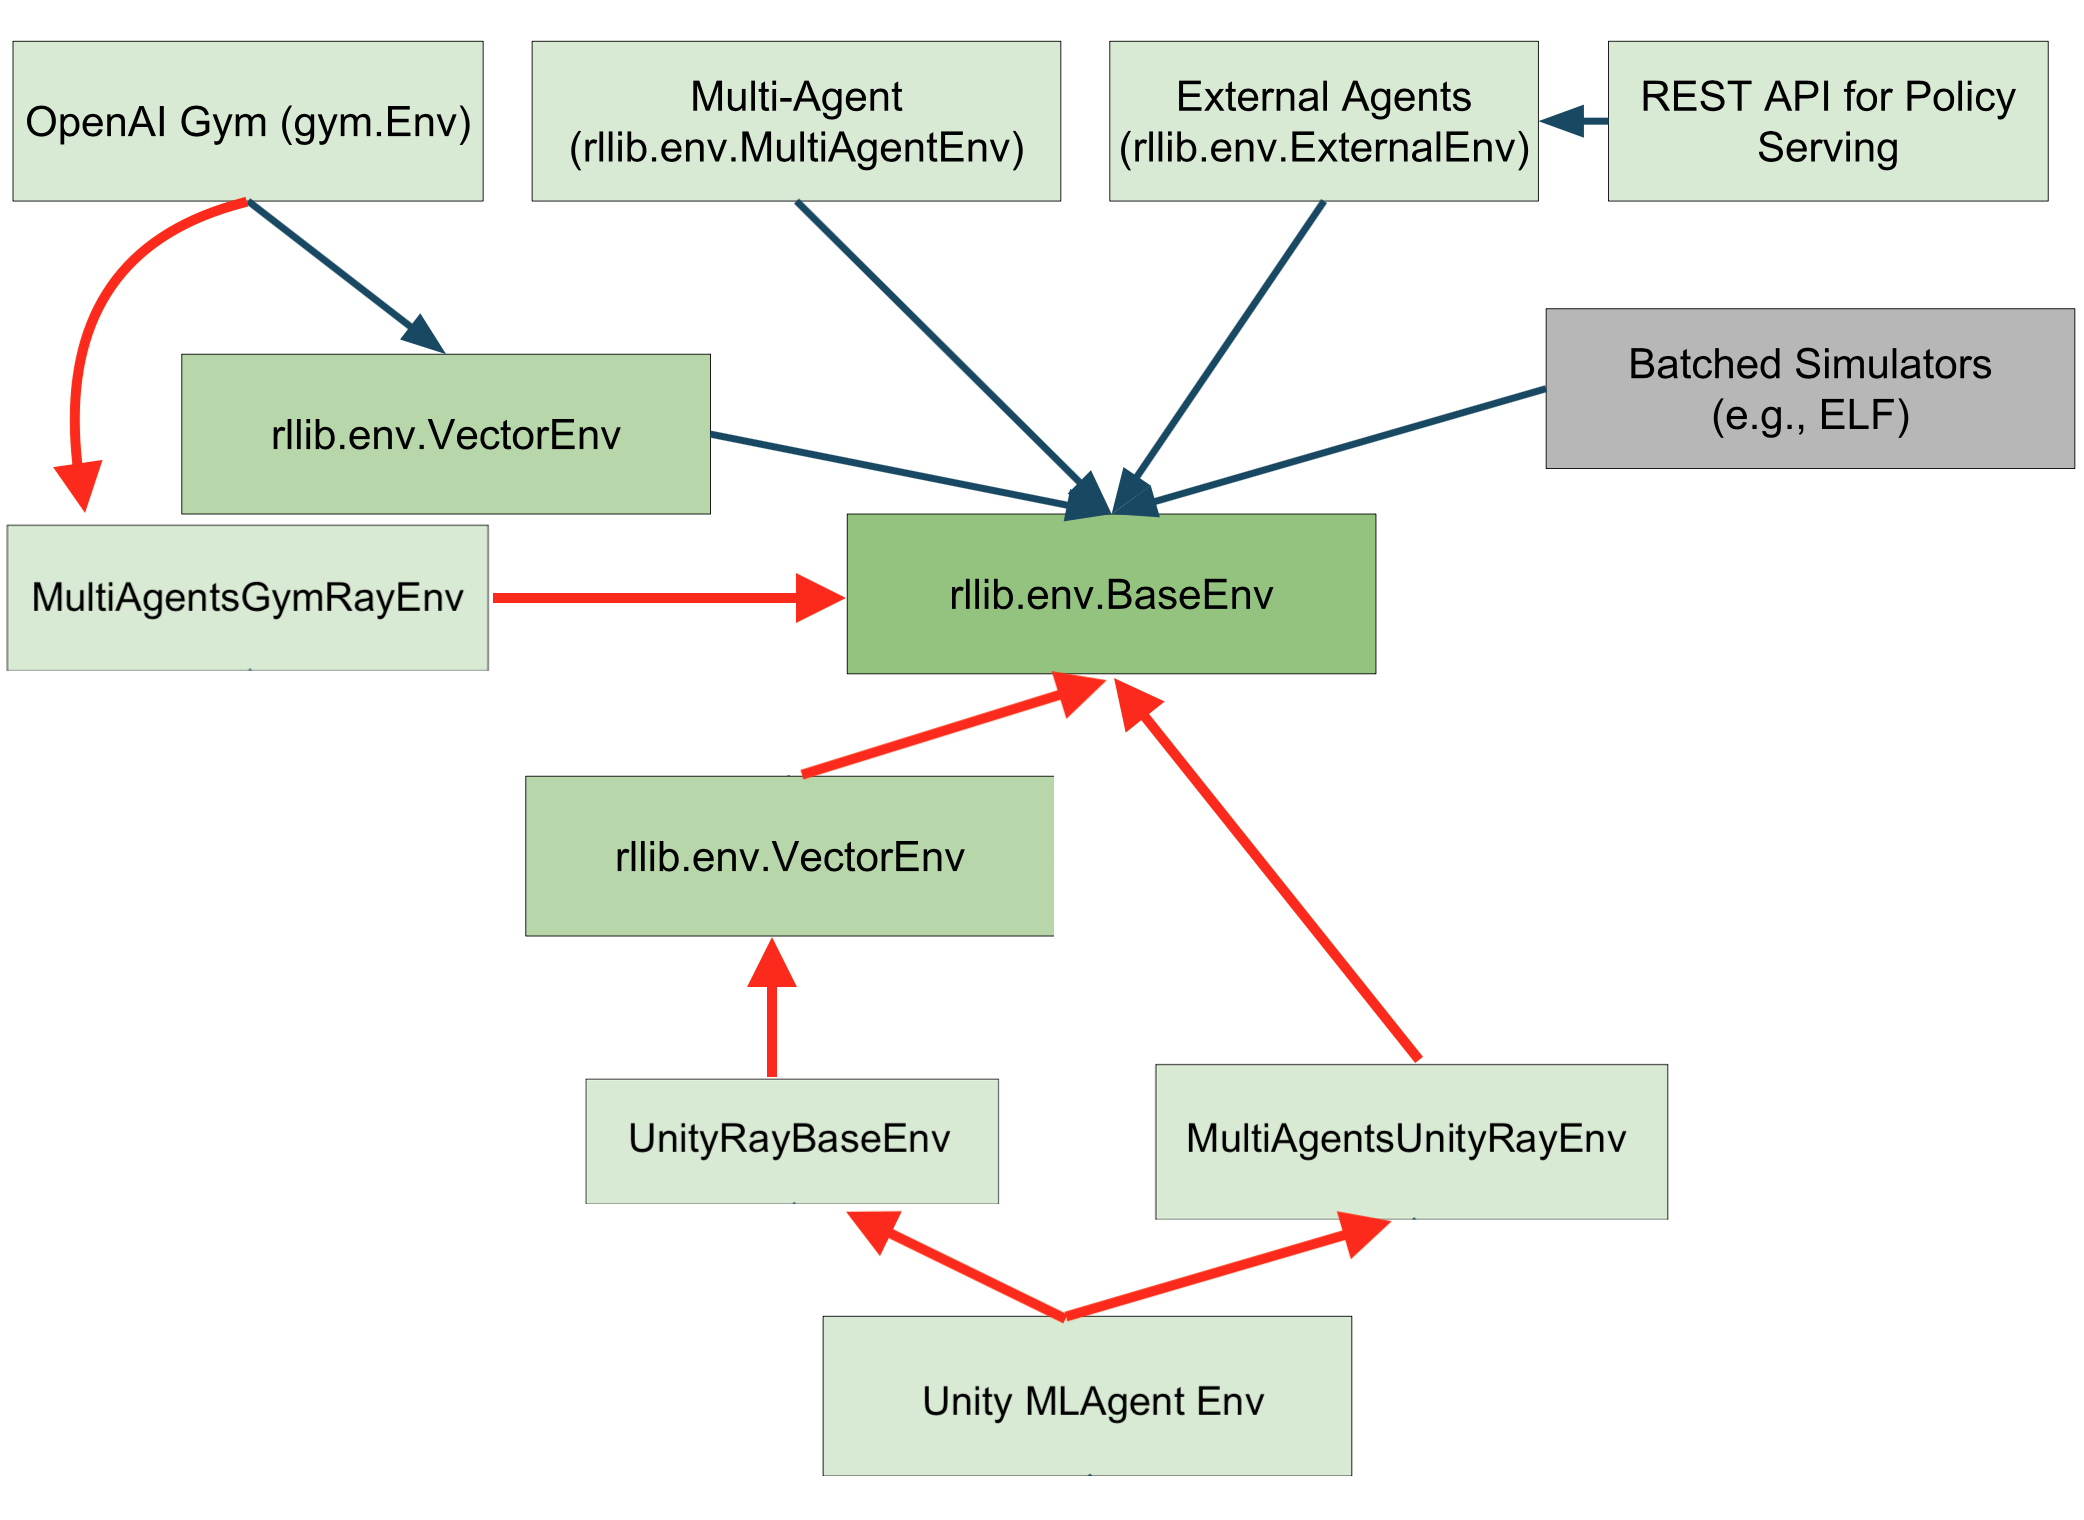
\includegraphics[width=0.7\linewidth]{figures/architecture/ray_envs.png}
	\caption{Our Custom Environments}
	\label{fig:ray_envs}
\end{figure}

% \clearpage

Custom environments implementations and methods are described below:

\textbf{UnityRayEnv}:\\
our base unity environment maps the observations and actions from unity mlagents toolkit to be compatible with Ray BaseEnv. Since unity mlagents deals with brains that control the agents and the environments we had to convert it to the required \colorbox{gray!20}{\texttt{observation\_space}} and \colorbox{gray!20}{\texttt{action\_space}} for ray env with the following methods:
\begin{itemize}
	\item \textit{\textbf{\colorbox{gray!20}{\texttt{\_\_init\_\_(self)}}}}: Create the unity environment from the unity build env, convert the observation and action spaces to be ray-compatible.
	\item \textit{\textbf{\colorbox{gray!20}{reset(self)}}}: Reset the environment's state. Returns observation.
	\item \textit{\textbf{\colorbox{gray!20}{step(self, action)}}}: Step the environment by one time-step. Returns observation, reward, done, info.
\end{itemize}

\textbf{MultiAgentsUnityRayEnv}:\\
this class inherit from both \colorbox{gray!20}{\textbf{UnityRayEnv}} and \colorbox{gray!20}{\textbf{MultiAgentEnv}}~\ref{fig:ray_multiagentenv}. The difference from the base environment is in both methods \textit{\textbf{\colorbox{gray!20}{reset(self)}}} and \textit{\textbf{\colorbox{gray!20}{step(self, \texttt{actions\_dict})}}}, where the reset function reset all the observations for each agent that exist in the environment and step function take a dictionary of actions corresponding for each action of a single agent. The same applies to \textbf{MultiAgentsGymRayEnv}.

\begin{figure}[!htb]
	\centering
	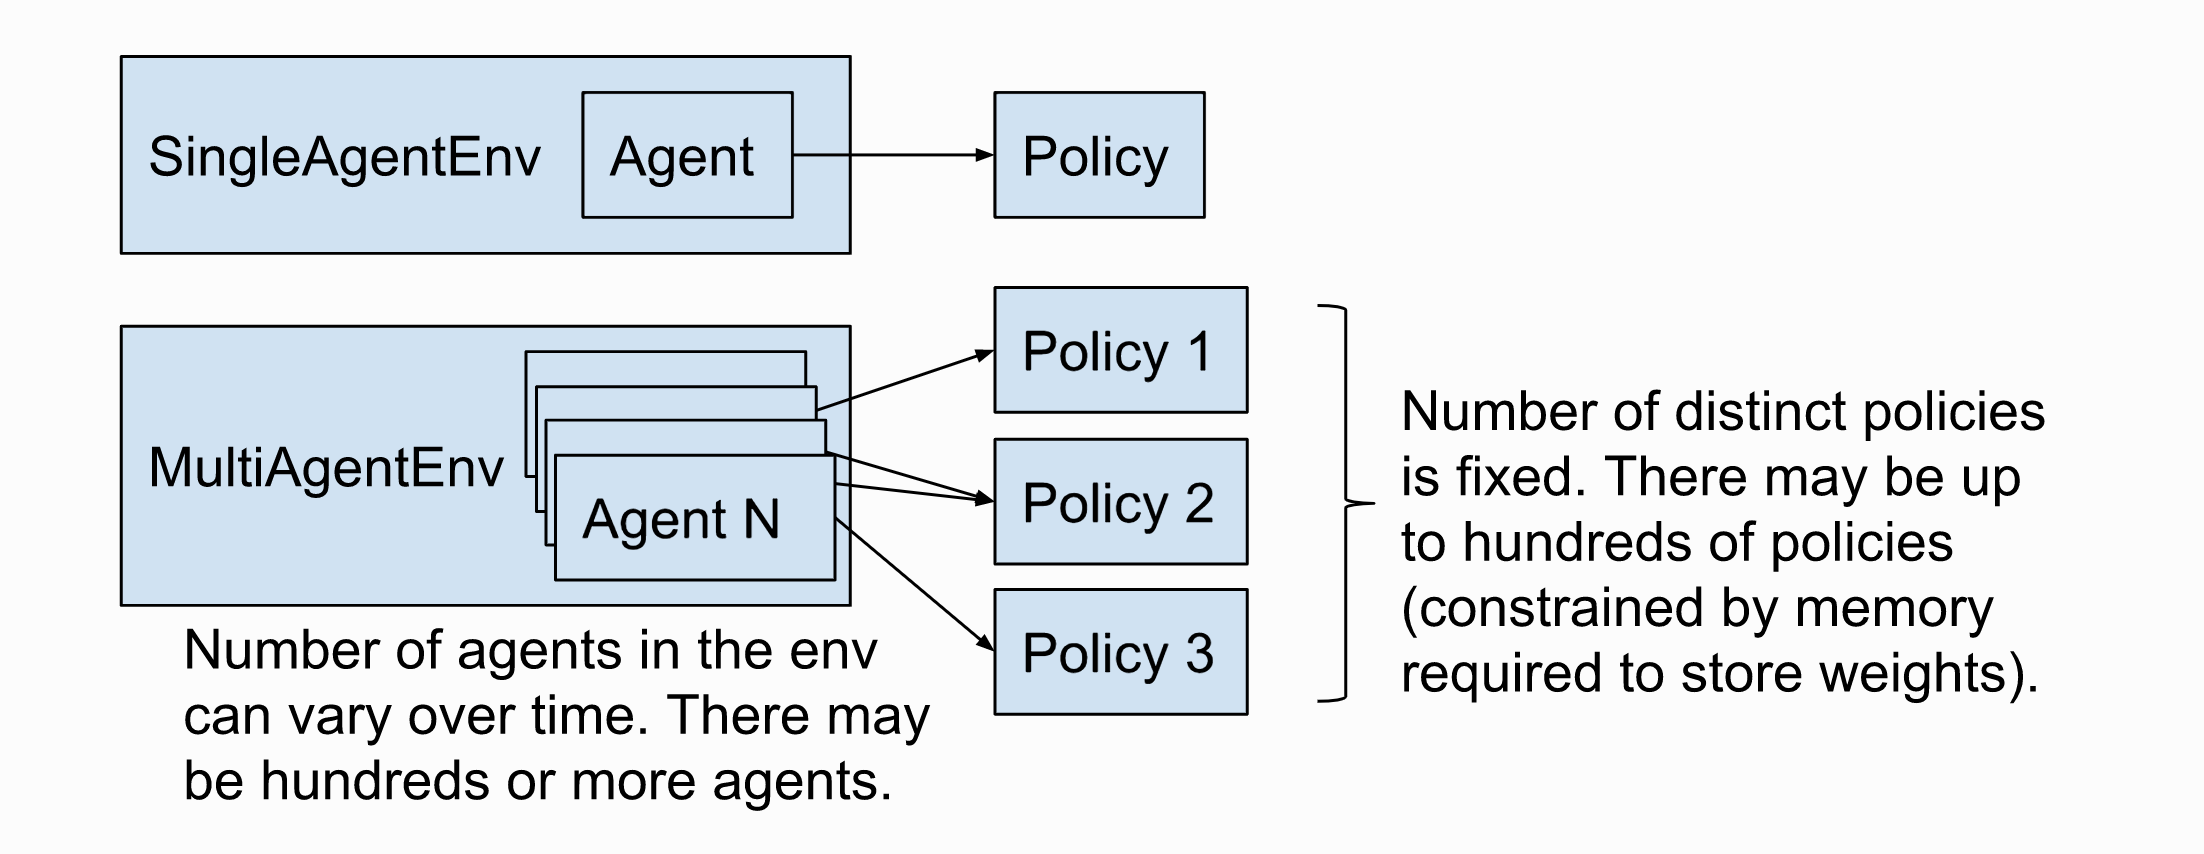
\includegraphics[width=\linewidth]{figures/architecture/ray_multiagentenv.png}
	\caption{Ray MultiAgentEnv}
	\label{fig:ray_multiagentenv}
\end{figure}

\section{Training Algorithms}

$\bullet$ \textit{\textbf{Proximal Policy Optimization (PPO):}} PPO is a policy gradient method introduced by openai which provides sampling data through interaction with the environment, and optimizing a surrogate objective function using stochastic gradient ascent. Its objective function enables multiple epochs of mini-batch updates. There are two primary variants of PPO: PPO-Penalty and PPO-Clip. In the conducted experiments, PPO-Clip is selected as PPO’s clipped objective supports multiple SGD passes over the same batch of experiences, enabling the use multi-GPU optimizer that pins data in GPU memory to avoid unnecessary transfers from host memory, substantially improving performance over a naive implementation. PPO scales out using multiple workers for experience collection, and also with multiple GPUs for SGD. In this way, it's possible to compare the naive implementation of PPO and the distributed version that support multi-GPU and multiple workers that can scale and improve the performance.

PPO-Clip doesn’t have a KL-divergence term in the objective and doesn’t have a constraint at all. Instead relies on specialized clipping in the objective function to remove incentives for the new policy to get far from the old policy. PPO is an on-policy algorithm, which can be used for environments with either discrete or continuous action spaces. Hence, the use of the PPO algorithm is suitable for our continuous space environments.

In the following figure~\ref{fig:ppo_algorithm}, a Pseudocode implementation for the used version of PPO.
\begin{figure}[!htb]
	\centering
	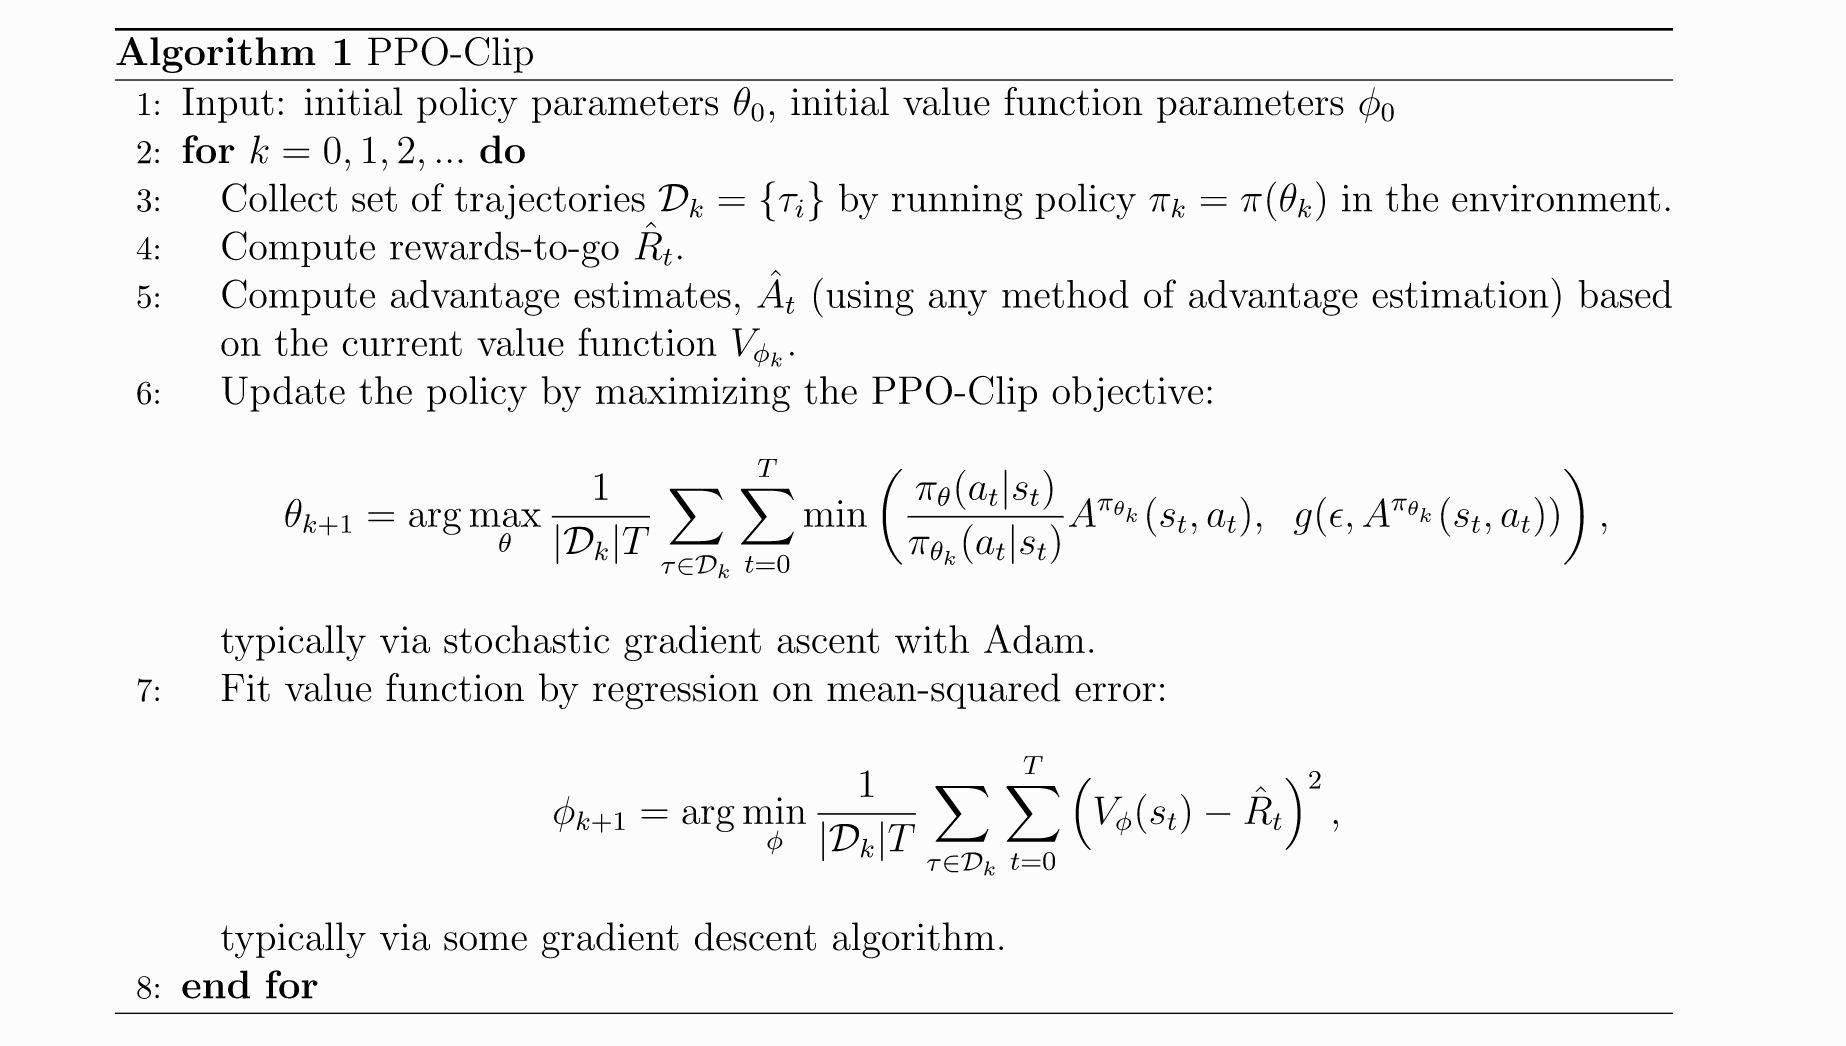
\includegraphics[width=\linewidth]{figures/ppo.png}
	\caption{PPO-Clip Pseudocode Implementation}
	\label{fig:ppo_algorithm}
\end{figure}


$\bullet$ \textit{\textbf{Distributed Prioritized Experience Replay (Ape-X):}} The idea behind Ape-X is that it decouples the learning from the actor, where allowing a central replay used only by the learner to employ prioritized experience replay. Another benefit is that it allows multiple actors to collect data in parallel (which may be used with different exploration strategies), ensuring both recency and diversity of data in the buffer. 

The architecture of the algorithm is well illustrated in figure~\ref{fig:apex_arch}, where there are multiple actors, each with its instance of the environment, generating experience, adding it to a shared experience replay memory, and compute initial priorities for the data. The (single) learner samples from this memory and updates the network and the priorities of the experience in the memory. The actors’ networks are periodically updated with the latest network parameters from the learner.

The learning algorithm, in general, follows the Q-learning style so that it can perform the off-policy update. 
The priorities are computed in each actor using local Q-values before sending data to the central replay, different from the original prioritized DQN, which initializes the priorities of new transitions to the maximum priority seen so far. This is because the original method would result in a myopic focus on the most recent data when there are a large number of actors. Local buffer also stores \(Q_{t}\) and \(Q_{t+n}\), which later will be used to compute priorities and discarded afterward. In contrast, this is not necessary when combining Ape-X with DDPG-style algorithms (a continuous-action policy gradient system based on DDPG), since the latter ones do not need to compute Q-functions when interacting with the environment. The Ape-X DPG setup is similar to Ape-X DQN, but the actor’s policy is now represented explicitly by a separate policy network, in addition to the Q-network.
In this way, a combination of Ape-X and DDPG is used for the experiments to support continuous spaces environments.

The detailed algorithm is described as in the following figures~\ref{fig:apex_algorithm}:
\begin{figure}[!htb]
	\centering
	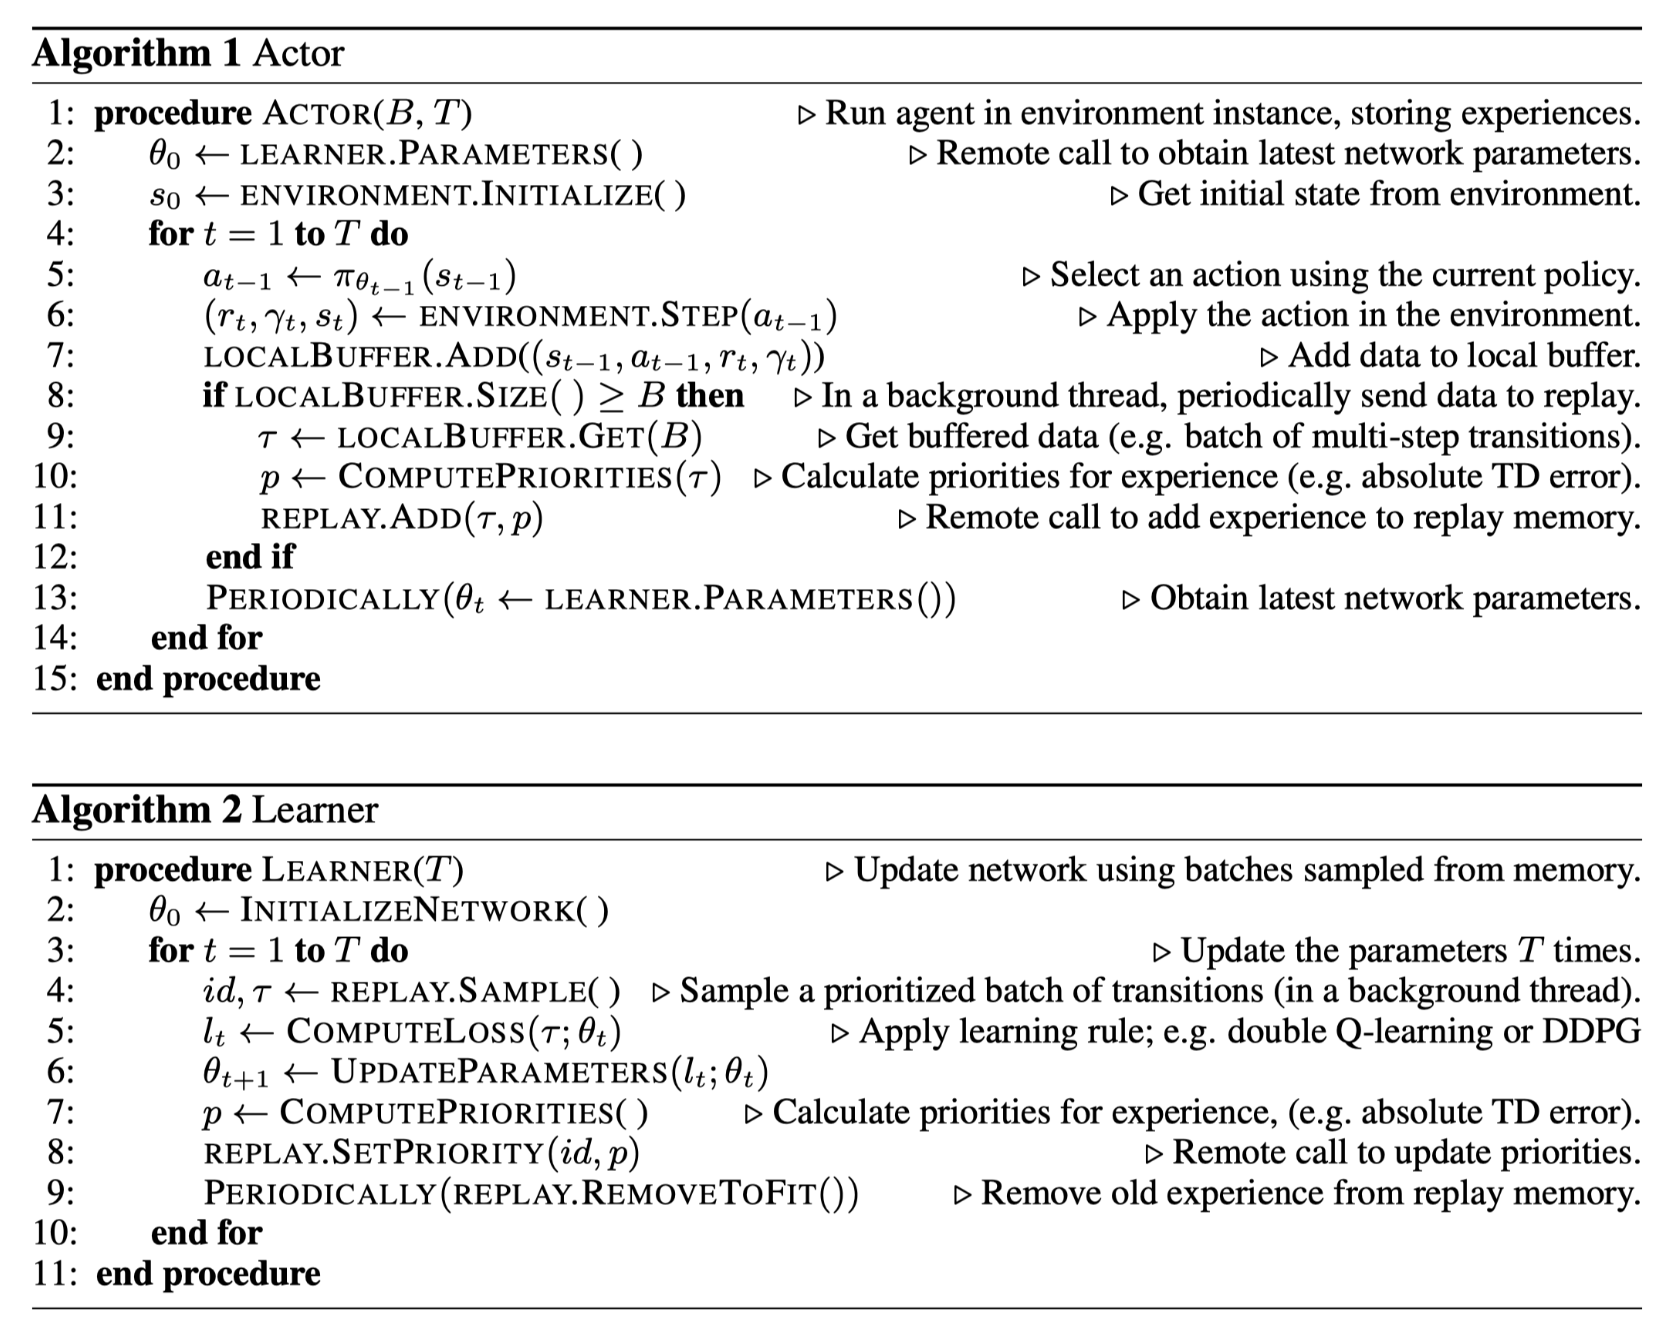
\includegraphics[width=0.7\linewidth]{figures/apex.png}
	\caption{Ape-X Pseudocode Implementation for both Actors \& Learner}
	\label{fig:apex_algorithm}
\end{figure}